
\documentclass{article}


%=========================================================================%
%
% Add optional packages. Some are almost essential.
%
%=========================================================================%

\usepackage[natbib=true,citestyle=authoryear,backend=bibtex]{biblatex}
\addbibresource{library.bib}
%\usepackage{natbib}
\usepackage[dvips]{graphicx}
\usepackage{lipsum}
\usepackage{listings}
\usepackage[utf8]{inputenc} % Input encoding and font encoding
%\usepackage[margin = 1in]{geometry} % Margins
\usepackage{setspace} % Setting the spacing between lines
\usepackage{amsthm, amsmath, amsfonts, mathtools, amssymb} % Math packages
\usepackage{sgame, tikz} % Game theory packages
\usetikzlibrary{trees, calc} % For extensive form games
\usepackage{pgfplots}
\usepackage{subfig} % Manipulation and reference of small or sub figures and tables
\usepackage{multirow,array}
%\usepackage[margin = 1in]{geometry} % Margins
\usetikzlibrary{calc}
\usetikzlibrary{matrix}
\usetikzlibrary{positioning}
\usepackage[mathscr]{euscript}
\usepackage{enumitem}
\usetikzlibrary{3d}
\usetikzlibrary{calc,fadings,decorations.pathreplacing}
\usepackage{bm,color}
\usepackage{makecell}
\usepackage{multicol}
\usepackage{float}
\restylefloat{table}
\usepackage{stackengine}
\usepackage{todonotes}
\usepackage{comment}
\usepackage{caption}
\usepackage[capitalize]{cleveref}
\usepackage{xcolor}


\newcommand\Under[2]{\strut%
  \setstackgap{L}{1.1\normalbaselineskip}%
  \setstackgap{S}{2pt}%
  \smash{\stackunder{#1}{#2}}%
}
\def\LA{\rlap{\scalebox{1.2}[1.5]{\kern2pt\raisebox{-.5pt}{$\leftarrow$}}}}
\def\RA{\rlap{\scalebox{1.2}[1.5]{\kern2pt\raisebox{-.5pt}{$\rightarrow$}}}}
\def\UA{\tclap{\scalebox{1.5}[2.2]{$\uparrow$}}}
\def\DA{\bclap{\scalebox{1.5}[2.2]{$\downarrow$}}}
%\renewcommand\arraystretch{1.5}
\renewcommand*{\nameyeardelim}{\addspace} % remove comma in text citations
\usepackage{pgf}
\usetikzlibrary{arrows}

\newcommand\addvmargin[1]{
  \node[fit=(current bounding box),inner ysep=#1,inner xsep=0]{};
}

% Theorems
\newtheorem{theorem}{Theorem}[section]
\newtheorem{corollary}[theorem]{Corollary}
\newtheorem{lemma}[theorem]{Lemma}
\theoremstyle{definition}

\newtheorem{definition}{Definition}[section]
\newtheorem{proposition}[definition]{Proposition}
%\newtheorem{theorem}[definition]{Theorem}
\newtheorem{notation}[definition]{Notation}
%\newtheorem{example}[definition]{Example}
%\newtheorem{corollary}[definition]{Corollary}
%\newtheorem{lemma}[definition]{Lemma}
\newtheorem{primary statistics}[definition]{Primary Statistics}
\newtheorem{auxiliary statistics}[definition]{Auxiliary Statistics}
%\newtheorem{definition}[theorem]{Definition}
%\newtheorem{proposition}[theorem]{Proposition}
%\newtheorem{notation}[theorem]{Notation}
\newtheorem{examplex}[theorem]{Example}
\newenvironment{example}
  {\pushQED{\qed}\renewcommand{\qedsymbol}{$\diamondsuit$}\examplex}
  {\popQED\endexamplex}

\lstset{
    literate={~} {$\sim$}{1}
}

\lstdefinestyle{DOS}
{
    backgroundcolor=\color{white},
    basicstyle=\scriptsize\color{black}\ttfamily
}

% \let\oldendexample\endexample
% \def\endexample{$\diamondsuit$\oldendexample}



%---------------------------%
% Argmax and Argmin
%---------------------------%
\DeclareMathOperator*{\argmax}{arg\,max} % argmax operator
\DeclareMathOperator*{\argmin}{arg\,min} % argmin operator


% Notation



\title{MC-AIXI-CTW Report}
\author{Elliot Catt, Suraj Narayanan, Arie Slobbe}
\begin{document}
\maketitle
\tableofcontents

\newpage

\section{Introduction}
We implement and test an approximation of the AIXI model \citep{hutter2005universal}. The AIXI model is a mathematical “solution” to the general reinforcement learning problem. That is, an AIXI agent solves the problem of maximising expected reward in an unknown computable environment that is potentially stochastic and partially observable. Unfortunately, the AIXI model is incomputable. A down-scaled (i.e. computable) version of AIXI is presented in \citep{veness2011monte} which is called Monte Carlo AIXI Context Tree Weighting, or MC-AIXI-CTW. Our work implements the agent design of Veness and colleagues with the aim to reproduce their experimental results on a variety of reinforcement learning domains.

The following subsections briefly introduce the three main components of the MC-AIXI-CTW agent. A complete description of the AIXI agent can be found in \citep{hutter2005universal}. The Monte Carlo component is described in \citep{kocsis2006bandit}, and the Context Tree Weighting method in \citep{willems1995context}.  Section 2 describes a variety of domains on which we tested our agent, section 3 describes our implementation of MC-AIXI-CTW and how to compile and run the code, and section 4 presents our experimental results on a variety of problem domains, and compares them with the results originally obtained by \citep{veness2011monte}.

\subsection{The AIXI agent}
AIXI is a Bayesian (``on-average'') optimality notion for general reinforcement learning agents. AIXI interacts with an unknown environment in cycles. In each cycle, the agent executes an action and in turn receives an observation and a reward. (when the environment is fully observable at all times, an observation is called a state; see figure 1). AIXI aims to choose actions that will on average lead to the best possible outcome. More precisely, AIXI maximises the expected sum of rewards over its lifetime.

Each time the agent takes an action, the environment responds by returning an observation reward pair. The agent processes the new observation-reward information and the next iteration begins with another action by the agent. In principle, the agent has access to its entire history of action-observation-reward cycles, and unlimited time to compute the next best action.  

\begin{figure}
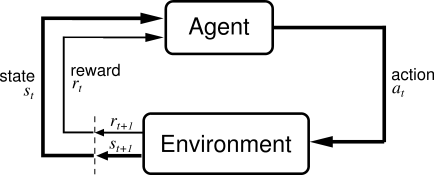
\includegraphics[width = 12cm]{suttonbarto_rl}
	\caption{\citep{sutton1998reinforcement}}
\end{figure}
 

Suppose the AIXI agent interacts with an environment in cycles $k=1,2, \ldots, m$. The agent chooses action $a_k$, subsequently the environment "chooses" (produces) an observation reward pair $o_kr_k$, and the next cycle begins. Over time, a history sequence $h=a_1o_1r_1 \ldots a_mo_mr_m$ is formed.

Agents are distinguished by how well they choose their actions in light of rewards received from the environment. In cycle $k$, the full AIXI model chooses its next action $a_k$ according to the following equation:

$$a_k \coloneqq \argmax_{a_k} \sum_{o_kr_k} \ldots \max_{a_m} \sum_{o_mr_m} (r_k+\ldots+r_m) \xi (o_1r_1 \ldots o_mr_m \mid a_1 \ldots a_m), $$

where $\xi (o_1r_1 \ldots o_mr_m \mid a_1 \ldots a_m)$ is a mixture environment model over a model class of chronological probability distributions. See \citep{hutter2005universal} for the full details of this model. Intuitively, the agent considers the sum of the total reward over all possible futures up to m steps ahead, weighs each of them by the complexity of (environments) consistent with the agent’s past that can generate the future, and then picks the action that maximises expected future rewards \citep{veness2011monte}. 

The alternating sum and max operators execute the (finite-horizon) expectimax operation, which is a classic result from sequential decision theory. Expectimax is responsible for planning a best course of action.

The mixture environment model is responsible for learning to predict future observations and rewards based on past experience. The technique is inspired by Solomonoff’s universal induction scheme. Initially, the mixture assigns greater weights to simple environment models. Each interaction cycle generates new evidence as to which models are more likely to be the “true” model of the environment. Models consistent with the evidence acquire increased weight (i.e. importance) in the decision procedure while inconsistent models are pruned away.

The AIXI agent requires an overwhelming number of computations to find its next action. The expectimax operation runs in exponential time with respect to lookahead $m$ and is computationally infeasible for all but the smallest values. Worse yet, the mixture environment model is not even finitely computable because the mixture is taken over an infinite set of environments. To deal with these issues, Veness et al. developed a computable approximation of AIXI. This approximation uses Monte Carlo Tree Search (MCTS) to approximate the expectimax operation and Context Tree Weighting (CTW) to maintain a mixture environment model. 

\subsection{Monte Carlo Tree Search}
Expectimax requires us to consider every possible future that can result from taking an action in the present. Again, this is computationally infeasible. Instead of considering every path through the future, Monte Carlo Tree Search (MCTS) samples as many paths as time and computation resources permit. An action with highly rewarding (simulated) futures is considered better than an action for which every sample returns nothing.

MCTS collects the outcomes of simulations in an iteratively expanding search tree.  \citep{kocsis2006bandit} developed a powerful heuristic which helps the agent focus its resources on useful parts of the tree. Actions with more simulations have better value estimates, so we must carefully consider which actions we care most about investing computational resources in. We prefer to spend resources on actions with high uncertainty about their real value, and/or with high probability of being the best action. These competing demands -- exploration of new actions, and exploitation of known good actions -- are balanced by taking a weighted average in such a way that total “regret” is minimised (see paper).

To illustrate, consider the problem of finding the best opening move in a game of tic-tac-toe. MC-AIXI-CTW runs a number of simulations to up to a pre-specified "search depth" into the future. The Context Tree Weighting method simulates the environment by taking prospective actions from the agent and return observation reward pairs, much like the environment would. In aggregate, the simulations yield an estimated win rate for each opening move. The agent subsequently chooses the opening move that had the highest win rate in its simulations.

\begin{figure}[h]
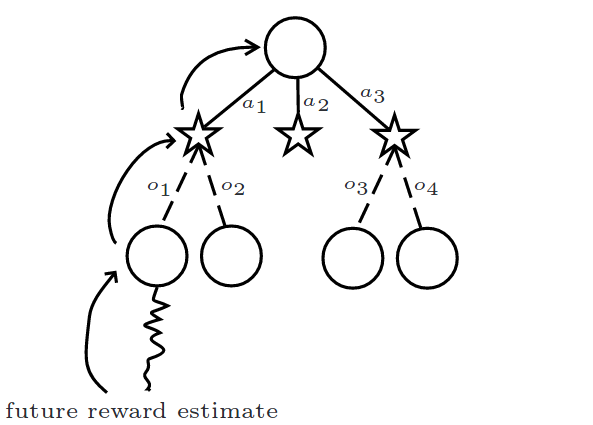
\includegraphics[width = 12cm]{mcts}
	\caption{\citep{veness2011monte}. Monte Carlo Tree Search collects the outcomes of simulations in an iteratively expanding search tree. The tree is composed of decision nodes (circles) and chance nodes (stars). These correspond to the alternating max and sum operations in the expectimax operation.}
\end{figure}

\subsection{Context Tree Weighting}
The Context Tree Weighting (CTW) method was initially proposed as a sequential universal compression method. CTW learns to identify patterns in a bit-sequence by performing Bayesian model averaging over all prediction suffix trees of maximum depth $D$. If the sequence generated by an $k$-order Markov process (that is, the probability of the next bit being 1 is conditioned on the last $k$ bits that were observed) and $k\leq D$ then CTW will converge to optimal prediction.

Several attributes make CTW a suitable approximator of universal Solomonoff induction:
\begin{itemize}
\item like Solomonoff induction, CTW maintains a mixture model over environments. The mixture converges to the true environment as evidence accumulates;
\item CTW assigns higher prior probability to simple models;
\item CTW covers the huge class of D-order Markov processes which contains many interesting and important environments; and
\item The running time of CTW is linear in the length of the input sequence, compared to exponential in the length of more na\"ive methods.
\end{itemize}

Each time the agent simulates taking an action, CTW is used to predict the subsequent observation reward pair. In the MC-AIXI-CTW implementation, every action, observation and reward is encoded as a string of bits. So in practice, to generate an observation reward pair, a number of steps are involved. CTW is asked to predict the next bit $b$ given the history sequence $h$, and subsequently the agent appends the predicted bit to the history sequence by setting $h \gets hb$. The agent predicts subsequent bits in this manner until they have appended to the original history $h$ a sequence of bits of length corresponding to an obseration reward pair. 

 
In this manner, the MC-AIXI-CTW agent uses the CTW method to simulate paths through the future in order to plan a best course of action.  By interacting with the environment, MC-AIXI-CTW acquires the training data for CTW to learn over time how to emulate the environment, making it an increasingly good predictor of the future. 

This convergence to the true environment works as follows.
Let $C_D$ denote the class of all prediction suffix trees of depth up to D, which are a form of variable order Markov models. We use $C_D$ as our environment class and we assume that the "true" environment $E^*$ is contained in $C_D$. To each $E \in C_D$ we assign a code with length $CL(E)$. We can think of this code as a compressed representation of the environment; simple environments have simple (short) codes and complex environments have complex (long) codes.

The mixture environment model $\xi$ from the AIXI model is approximated by 
\begin{equation} \label{eq1}
\begin{split}
\xi (o_1r_1 \ldots o_mr_m \mid a_1 \ldots a_m) &\approx  P_{CTW}(o_1r_1 \ldots o_mr_m \mid a_1 \ldots a_m) \\
 & = \sum_{E \in C_D} P(E) P(o_1r_1 \ldots o_mr_m \mid E, a_1 \ldots a_m) \\ 
 & = \sum_{E \in C_D} 2^{-CL(E)} P(o_1r_1 \ldots o_mr_m \mid E, a_1 \ldots a_m).
\end{split}
\end{equation}

% Explain how convergence to true occurs
The $2^{-CL(E)}$ factor causes simple environments to have an outsize contribution on the output value $P_{CTW}$. The factor $P(o_1r_1 \ldots o_mr_m \mid E, a_1 \ldots a_m)$ approaches zero when the ``real" environment $E^*$ produces observation reward pairs $o_1r_1 \ldots o_mr_m$ that we would not likely observe if $E$ were the true environment. Hence, over time the $P(o_1r_1 \ldots o_mr_m \mid E^*, a_1 \ldots a_m)$ term that corresponds to the real environment $E*$ will dominate the sum. 


\section{Overview of implemented domains}
\subsection{Kuhn Poker}
Kuhn Poker is a simplified version of poker that was introduced in \citep{kuhn1950simplified}. It involves a deck of 3 cards (King, Queen, Jack). First the cards will be given out, and each player bets 1, then the opponent will choose to bet or pass, after looking at his card, the agent will then choose to bet or pass. If the actions taken are equal (both bet or both pass) then the player with the higher card wins the round (King$>$Queen$>$Jack). If instead the agent chose to pass, the opponent wins the round. If the opponent passed then the agent bet 1, the opponent then has the choice to bet or pass again, if they pass the agent wins, if they bet then the player with the highest card wins. \\

The opponent will always play the Nash Strategy. To represent this at the start of the round the opponent chooses an $\alpha\in [0,\frac{1}{3}]$ at random. If they drew a Jack, they will bet with probability $\alpha$. If they drew a queen they will bet with probability 0. If they drew a king they will bet with probability $3\alpha$. If there is a second round of betting, they will choose to bet with probability $\alpha+\frac{1}{3}$ regardless of their card. \\

If the agent wins, they get reward equal to the number of chips in play. If the agent loses they will get a reward equal to the negative of the number of chips they bet. In True Kuhn Poker, that is exactly as detailed in \citep{kuhn1950simplified} the reward for the agent is the number of chips the opponent put in.


\subsection{Biased Rock Paper Scissors}
Biased Rock Paper Scissors is very similar to regular rock paper scissors, with an exception in how the opponent chooses to play. Both the agent and the opponent will choose either Rock, Paper or Scissors. As per usual, Rock beats Scissors, Paper beats Rock, Scissors beats Paper. If the agent beats the opponent, the agent will receive a reward of 1. If the agent loses it will receive a reward of -1. If it is a draw, meaning both opponent and agent make the same choice, then the agent receives a reward of 0. The opponent repeats its choice of the previous round if it resulted in a win, and picks a random move otherwise. 

\subsection{Coin Flip}
The Coin Flip is a very simple environment where the agent will choose heads or tails. Then a biased coin with probability $p$ for heads and $1-p$ for tails will be flipped. If the agent guesses correctly it will receive reward of 1, if not it will receive a reward of 0.

\subsection{Extended Tiger}
Extended tiger is a simple game where the agent begins sitting on a chair, in front of two doors. Behind one door is a tiger, behind the other is gold. While sitting the agent has the choice to stand or listen to the door. If the agent listens they will make a correct observation about which door the tiger is behind with a probability of 0.85, and observe the wrong door with probability 0.15. Once standing the agent can open door 1 or open door 2. If the agent opens the door with the gold they receive a reward of 30, and if they open the door with the tiger they receive a reward of -100. If the agent stands up while sitting down or listens while sitting down they will receive a reward of -1. Any invalid action the agent performs yields a reward of -10.

\subsection{Partially Observable Pacman}
Partially observable pacman (POcman) is a version of the 17x19 pacman game where the agent controlling Pacman cannot observe the whole space. Instead, pacman can detect: if there are walls around him; if he can see a ghost in the four directions around him; if there are is a food pellet within 2, 3, and 4 of his location; if he can see a food pellet in any of the four directions; and if he has the power pill or not. The ghosts will move randomly, unless they are within a manhattan distance of 5 or less, in which case they will try to move towards him. The agent receives a reward of -1 for every move it makes, -10 for hitting a wall, +10 for collecting a food pellet, -50 if touched by a ghost, and +100 when it completes the level by collecting all pellets.

\subsection{Tic Tac Toe}
Tic Tac Toe is an adversarial fully observable deterministic game played on a 3 by 3 board. It begins with the agent placing a ‘X’ on one of the places on the board, the opponent then places an ‘O’ on another place. This continues until there is a horizontal, vertical or diagonal line of 3 ‘X’s or ‘O’s on the board, at which point the game is over and the player who played the line wins. If the board is full and there is no winner, then the game is a draw. If the agent attempts to place an ‘X’ on a place that already has a piece he will penalized by -3 reward. If the agent loses the game, they get a reward of -2. If the agent wins the game they get a reward of 2, and if the agent draws the game it will get a reward of 1. The opponent will always play in a random available spot.


\section{Overview of agent program}

The MC-AIXI-CTW agent program is composed of several components. Each is briefly presented in the following overview. More comprehensive documentation is provided in the source files themselves.

% The \textbf{conf} folder contains configuration settings for each of the implemented environments, which are kept in the environments folder. 

% The folder named \textbf{common} contains definitions of various functions and constants that are used across the program. 

% The file \textbf{main.cpp} reads and parses configuration files, calls various initialisation code, and contains the main agent/environment interaction loop.

% The \textbf{AIXI} folder holds the Agent class which contains high-level code relating to action selection, model prediction, observation decoding, and action encoding.

% The \textbf{MCTS} folder contains the SearchTree and SearchNode classes which implement the UCT algorithm for planning optimal actions within the environment. Veness et al. reconstruct a search tree from scratch at every new cycle. In contrast, our method employs a prune method to reuse as many computations as possible from the previous cycle.

% The \textbf{CTW} folder contains the CTNode and ContextTree classes which implement the CTW method for predicting and simulating the environment.

\begin{itemize}
    \item \textbf{AIXI} The AIXI module has four main functions: 
    \begin{itemize}
        \item \textbf{(d)encode}: Decodes and encode the reward, actions and percepts of the agent with the environment.
        \item \textbf{update}: Updates the model based on the updated and generated percepts.
        \item \textbf{initialisation}: Initialises the agents parameters: History size, number of simulations/actions, number of observation and reward bits.
        \item \textbf{planning}: The planner from the search tree returns a planned action.
    \end{itemize}
    \item \textbf{MCTS} \begin{itemize}
        \item \textbf{search tree}: The search tree is created, pruned, and search through.
        \item \textbf{produce action}: The best action is chosen from the search tree.
    \end{itemize} 
    \item \textbf{CTW}\\
    The CTW module has two main functions: 
    \begin{itemize}
        \item \textbf{update}: Takes care of updating and/or reverting the context tree. Update handles both by means of a flag variable that indicates the operation that need to be performed.
        \item \textbf{genNextSymbolsAndUpdate}: Generates the symbols for the next percept and updates the tree with them.
    \end{itemize}
    Detailed documentation of the other functions are given in the header file.\\

    \textbf{Implementation Details}
    \begin{itemize}
        \item \textbf{Numerical Stability:} All the probability related calculations are done in log-space to avoid under-flow issues.
        \item \textbf{Efficient Node Creation:} Nodes are created dynamically when requested. This allows for slow memory growth.
        \item \textbf{Efficient Node Deletion:} Nodes created during MCTS simulations are deleted, thereby reclaiming memory allocated during MCTS search.
        \item \textbf{Generic Update:} The update method is equiped with an operation flag so that the same infrastructure can be re-used to perform \textit{revert} operation as well.
        \item \textbf{Built-in Sanity Checks:} The code has built-in sanity-check that take palce every update/revert operation. The code checks for invalid probability values, and invalid reverts.
    \end{itemize}
\end{itemize}


\subsection{Software Architecture}

\begin{figure}[h]
    \centering
    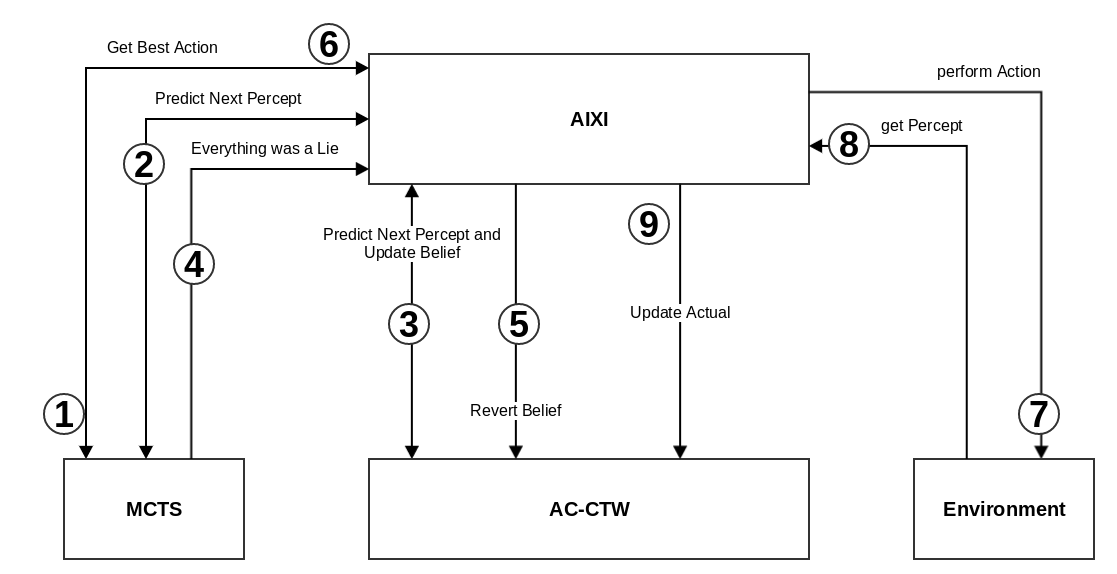
\includegraphics[height=5.5cm]{soft_arch_crop}    
\end{figure}

Our implementation of MC-AIXI-CTW was designed keeping modularity and extensibility in mind. The figure above shows the components and the interaction between them. Logically the system is split into four parts. 
\begin{itemize}
    \item \textbf{Agent: } AIXI
    \item \textbf{Planner: } MCTS
    \item \textbf{Model-learner: } CTW
    \item \textbf{Environment: } TicTacToe/Pacman/BiasedRPS/...
\end{itemize}

The interaction between the modules is designed in such a way that each component is loosely coupled. This allows any component adhering to AIXI's interface to be plugged in without any change being effected in other module.

\subsubsection*{Agent-Environment Interaction Workflow}
\begin{enumerate}
    \item AIXI asks MCTS for the best action.
    \item MCTS in turn asks AIXI to predict what the next percept would be.
    \item AIXI asks CTW for the next percept, and updates the CTW with the percept. AIXI sends the percept to MCTS.
    \item MCTS tells the agent that it has finished planning, and its time to revert the prediction.
    \item AIXI tells CTW to revert the prediction.
    \item MCTS returns the next best action to AIXI.
    \item AIXI performs the action on the Environment.
    \item Environment returns a percept to AIXI.
    \item AIXI updates the CTW with the percept.
\end{enumerate}


\subsection{How to compile and run}
\subsubsection*{Linux/Mac OS}
Extract the source files into a folder 
\begin{lstlisting}[style=DOS]
 ~/mc-aixi-ctw 
\end{lstlisting}
 and execute in the terminal:
 
\begin{lstlisting}[style=DOS]
cd ~/mc-aixi-ctw
make all
./bin/aixi -c /conf/coinflip.conf
\end{lstlisting}

\subsubsection*{Windows (Cygwin)}
Extract the source files into a folder for example
\begin{lstlisting}[style=DOS]
 /cygwin/c/mc-aixi-ctw 
\end{lstlisting}
and execute the command (in Cygwin)
\begin{lstlisting}[style=DOS]
cd mc-aixi-ctw
make all
/bin/aixi.exe -c /conf/coinflip.conf
\end{lstlisting} 

The file coinflip.conf may be replaced with any other file in the conf folder. 
After execution, the two files logfile.log and logfile.csv will contain data on the agent’s actions and performance. Additionally, the command
\begin{lstlisting}[style=DOS]
./bin/aixi -h
\end{lstlisting}
or if using windows (cygwin)
\begin{lstlisting}[style=DOS]
/bin/aixi.exe -h
\end{lstlisting}
can be executed to find for more details on how to run the program.




\section{Experimental Results}

Our objective is to test the agent's learning capability in an environment with no prior knowledge. The learnt policy is evaluated at the end of the training phase. For the environments, some are easy such as Biased Rock-Paper-Scissors, and Kuhn-Poker. The other environments TicTacToe, Pacman, Extended Tiger are harder games to learn. In each experiment in each domain we chose a CTW Depth, a Horizon, an Exploration, and Exploration Decay and a Number of Cycles. For each set of chosen parameters we run 4 experiments of our agent on the given domain with the given parameters. We indexed each parameter set by experiment ID. \\

The parameters were chosen so that we had a balance between the parameters used in \citep{veness2011monte} and computational efficiency. The exploration and exploration decay were chosen so that after the number of cycles the exploration would be $10^{-5}$. For most environments we fixed the horizon and increased the CTW depth. This was done to see what influence the choice of CTW depth had on the results. \\

Our experimental results for the environments are as follows, we use the following notation,
 \begin{align*}
     D &= \text{ CTW Depth} \\
     m &= \text{ Horizon} \\
     \epsilon &= \text{ Exploration} \\
     \gamma &= \text{ Exploration Decay} \\
     \text{Cycles }\times 10^3 &= \text{ Number of cycles }  \\
     \text{E\underline{ } } &= \text{ Intermediate Evaluation}
 \end{align*}
Next are the parameters used in each environment, with the average reward of each set of parameters in the environment. For each environment we graphed each configuration value compared with each other. Additionally for each environment we graphed of the performance of our agent over time, compared with intermediate evaluation of our agent, the agent in \citep{veness2011monte} and a random agent. In each graph the shaded region is the standard deviation from the 4 experiments run for that chosen ste of parameters.



\newpage

\subsection{Biased Rock Paper Scissors}
\begin{tabular}{|l|l|l|l|l|l|l|}
\hline \centering
 Experiment ID& D & m & $\epsilon$ & $\gamma$ & Cycles & Average Reward \\ \hline
BRPS-1        & 32        & 4           & 0.999       & 0.9995            & 30     & 0.2293375        \\ \hline
BRPS-2        & 96        & 8           & 0.999       & 0.9991            & 12     & 0.2419375       \\ \hline
BRPS-3        & 256       & 4           & 0.999       & 0.9991            & 13     & 0.21425        \\ \hline
BRPS-4        & 256       & 8           & 0.999       & 0.999             & 7      & 0.246525  \\ \hline  
E\underline{ }BRPS        & 256       & 8           & 0.999       & 0.999             & 9      & N/A  \\ \hline      
\end{tabular} 


 \begin{figure}[h]
 \centering
    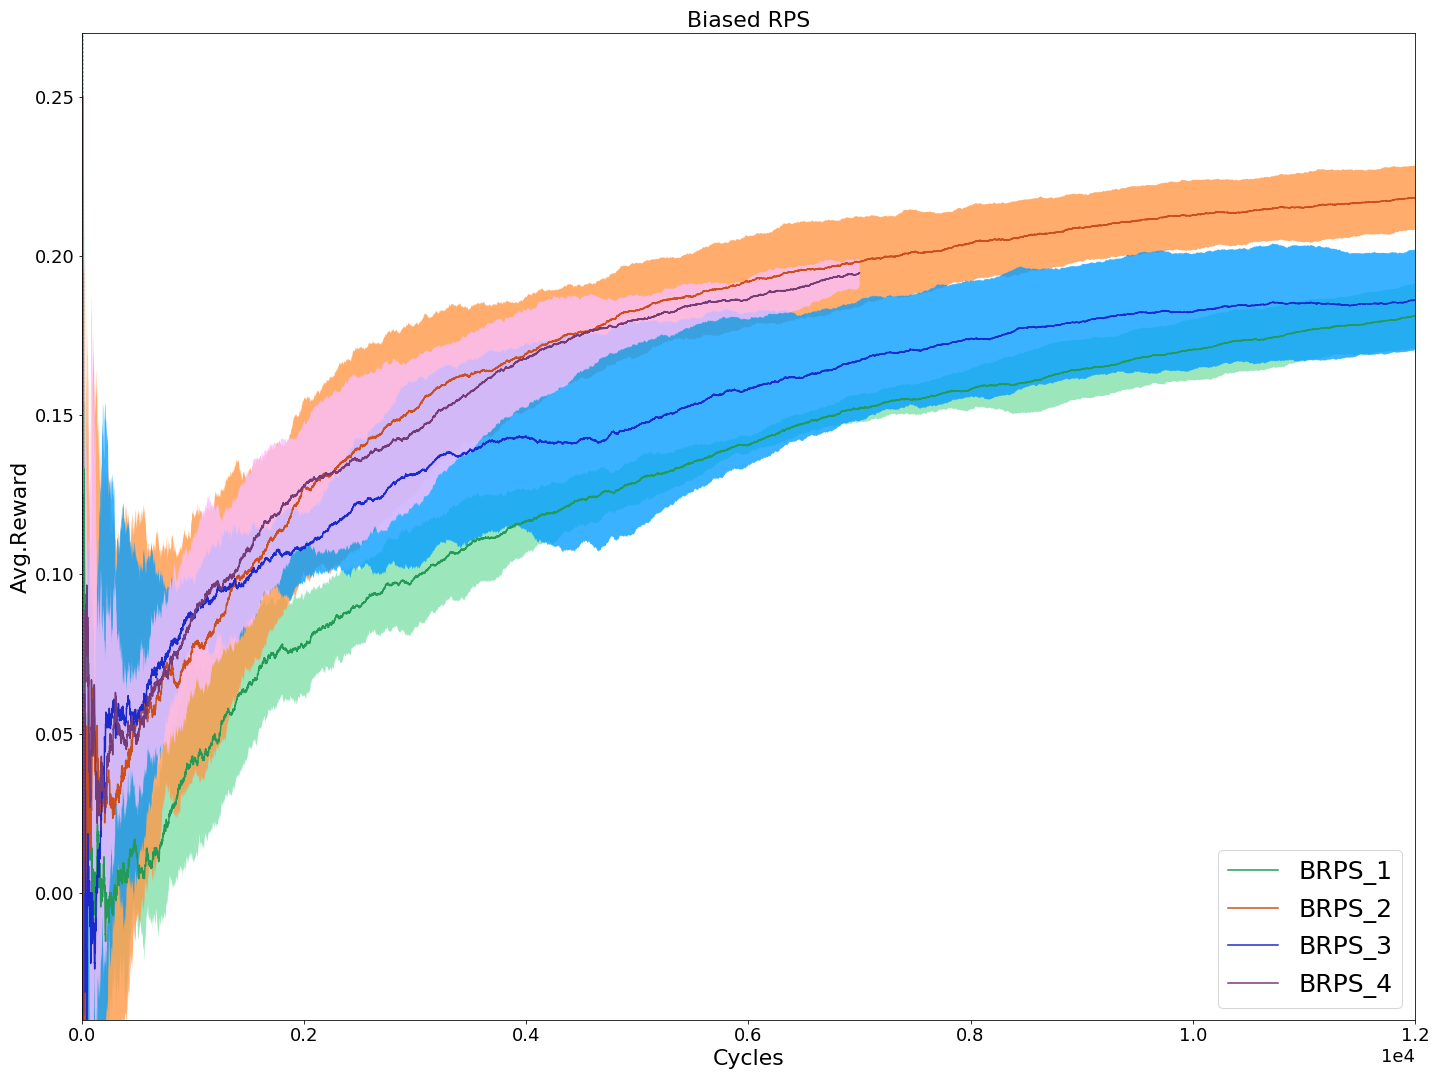
\includegraphics[width=9.1cm]{4_Biased_RPS}
\end{figure}

\begin{figure}[h]
\centering
    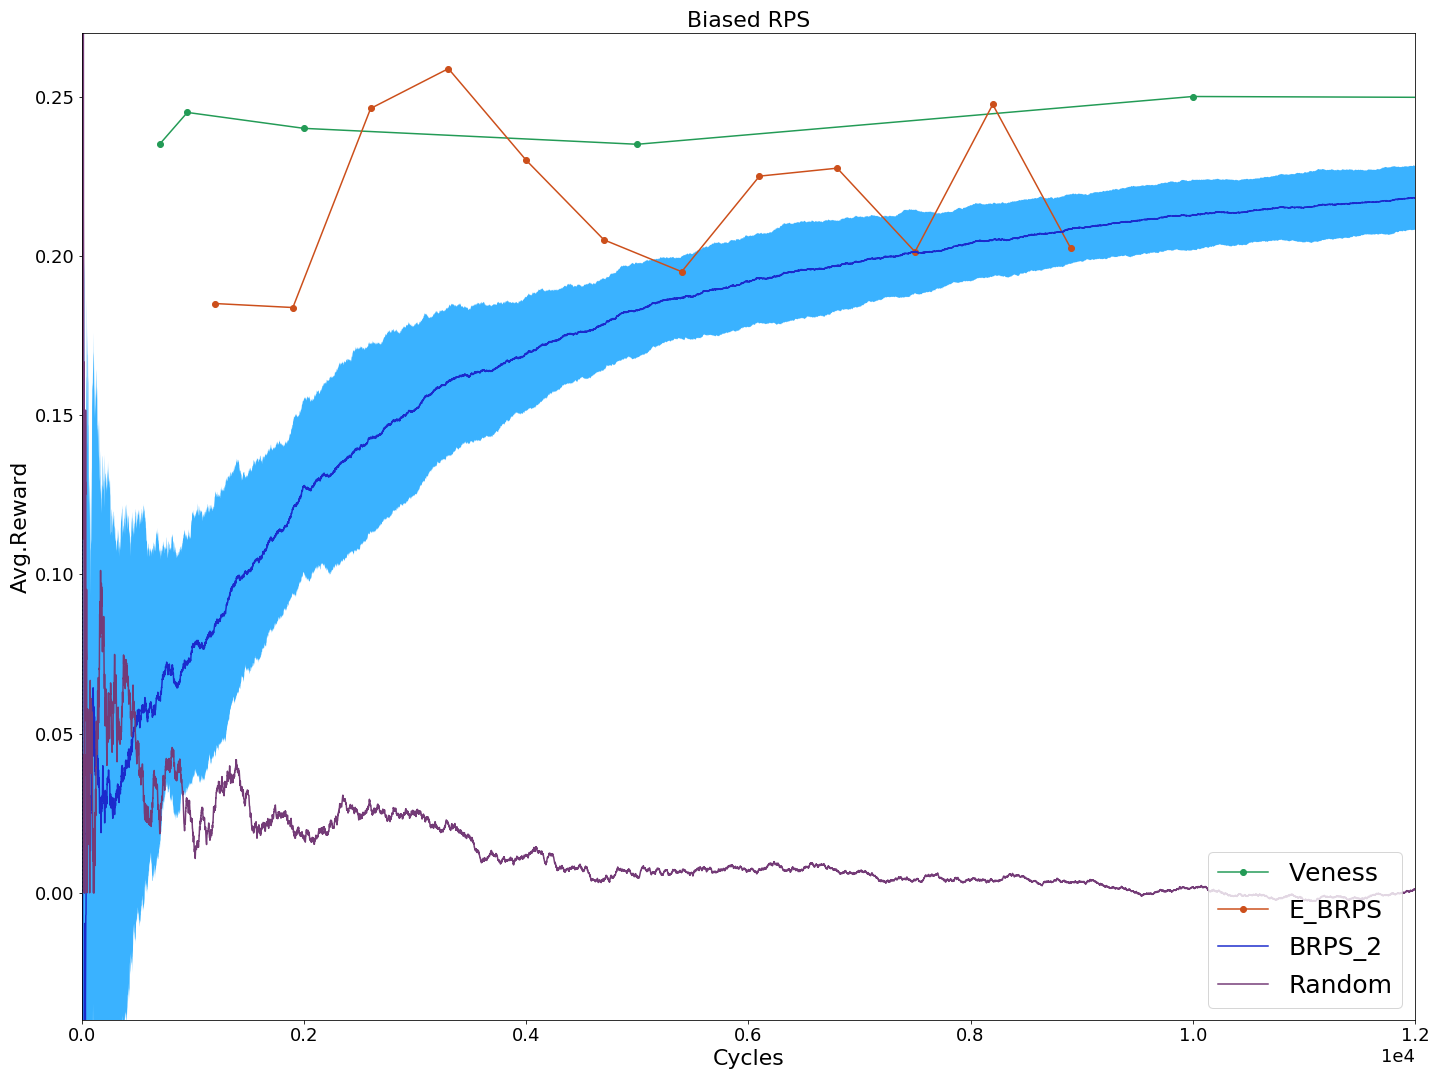
\includegraphics[width=9.1cm]{Biased_RPS}
\end{figure}

Compared to the random agent, our agent performed superiorly. Compared to \citep{veness2011monte} our agent performed similarly.

\newpage

\subsection{Kuhn Poker}

\begin{tabular}{|l|l|l|l|l|l|l|}
\hline \centering 
  Experiment ID& D & m & $\epsilon$ & $\gamma$ & Cycles & Average Reward \\ \hline
KPKR-1  & 42        & 2           & 0.99        & 0.9999            & 2000   & 1.2024625        \\ \hline
KPKR-2  & 96        & 4           & 0.9999      & 0.9995            & 24     & 1.258875         \\ \hline
KPKR-3  & 256       & 4           & 0.999       & 0.9991            & 13     & 1.23595         \\ \hline
E\underline{ }KPKR  & 96       & 4           & 0.9999       & 0.9995            & 30     & N/A         \\ \hline
%Kuhn Poker  & 512       & 8           & 0.9999      & 0.999             & 7      &               
\end{tabular} 


 \begin{figure}[h]
 \centering
    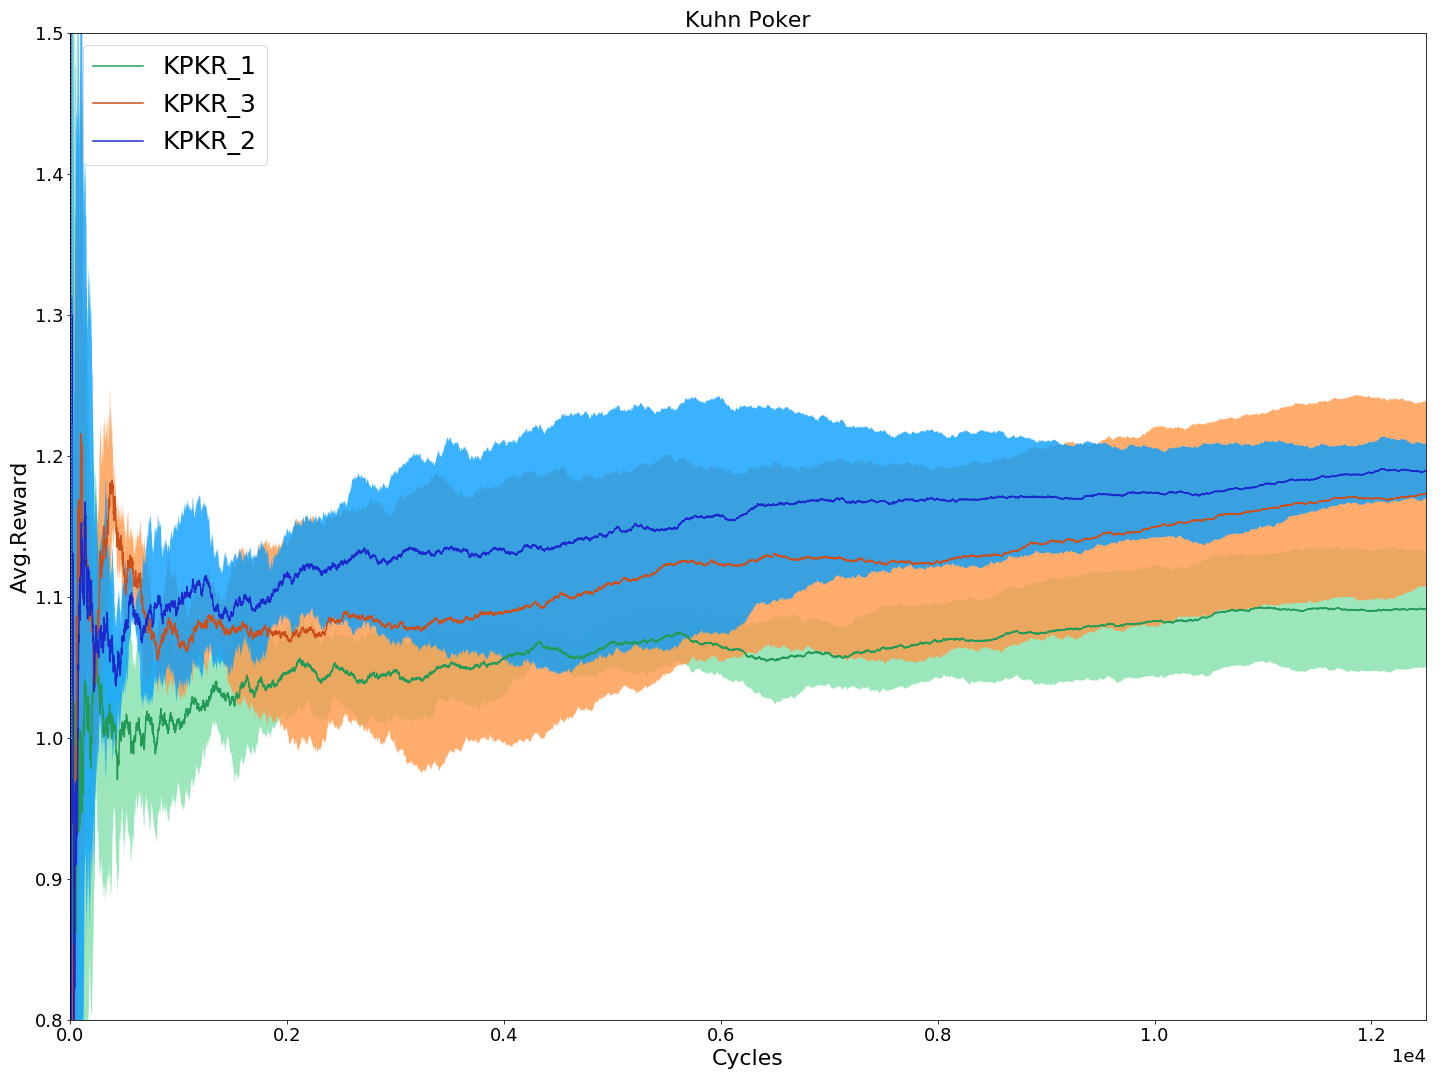
\includegraphics[width=9.1cm]{4_Kuhn_Poker}
\end{figure}

 \begin{figure}[h]
 \centering
    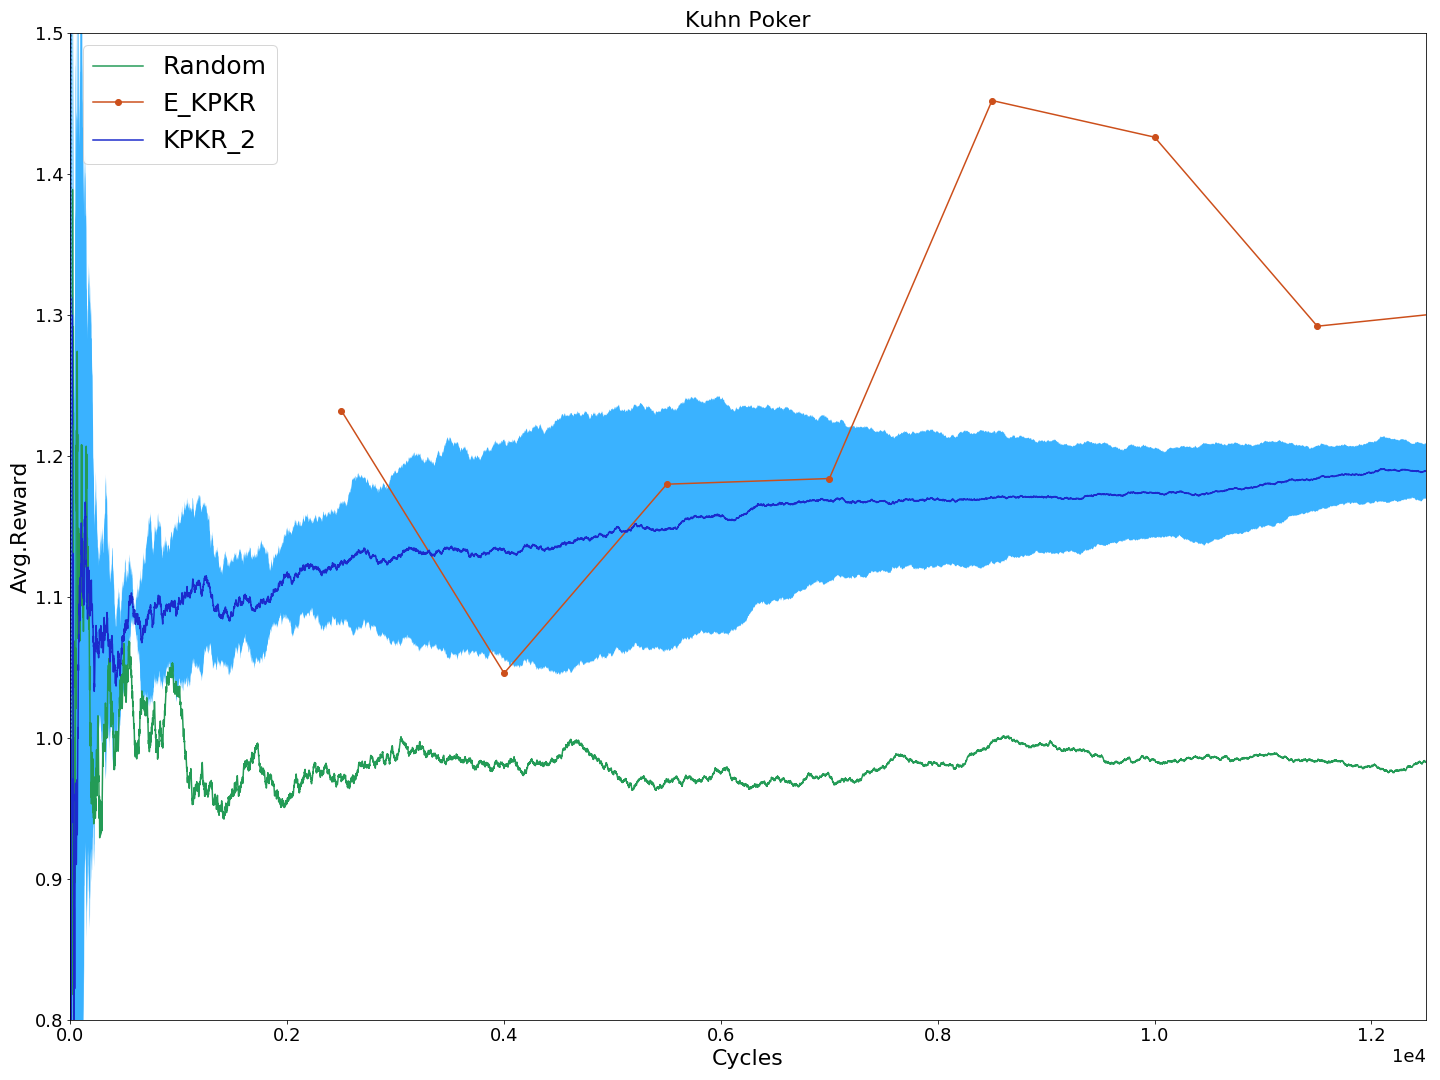
\includegraphics[width=9.1cm]{Kuhn_Poker}
\end{figure}

Compared to the random agent, our agent performed superiorly. We did not compare with \citep{veness2011monte} since they used Kuhn Poker.

\newpage

\subsection{True Kuhn Poker}
\begin{tabular}{|l|l|l|l|l|l|l|}
\hline \centering
 Experiment ID& D & m & $\epsilon$ & $\gamma$ & Cycles & Average Reward \\ \hline
TKPKR-1  & 42        & 2           & 0.99        & 0.9999            & 2000   & 0.0719        \\ \hline
TKPKR-2  & 96        & 4           & 0.9999      & 0.9995            & 24     & 0.01415         \\ \hline
TKPKR-3  & 256       & 4           & 0.999       & 0.9991            & 13     & 0.0611         \\ \hline
TKPKR-4  & 512       & 8           & 0.9999      & 0.999             & 7      & 0.056      \\ \hline 
E\underline{ }TKPKR  & 96       & 4           & 0.9999      & 0.9995             & 30      & N/A      \\ \hline        
\end{tabular} 

 \begin{figure}[h]
 \centering
    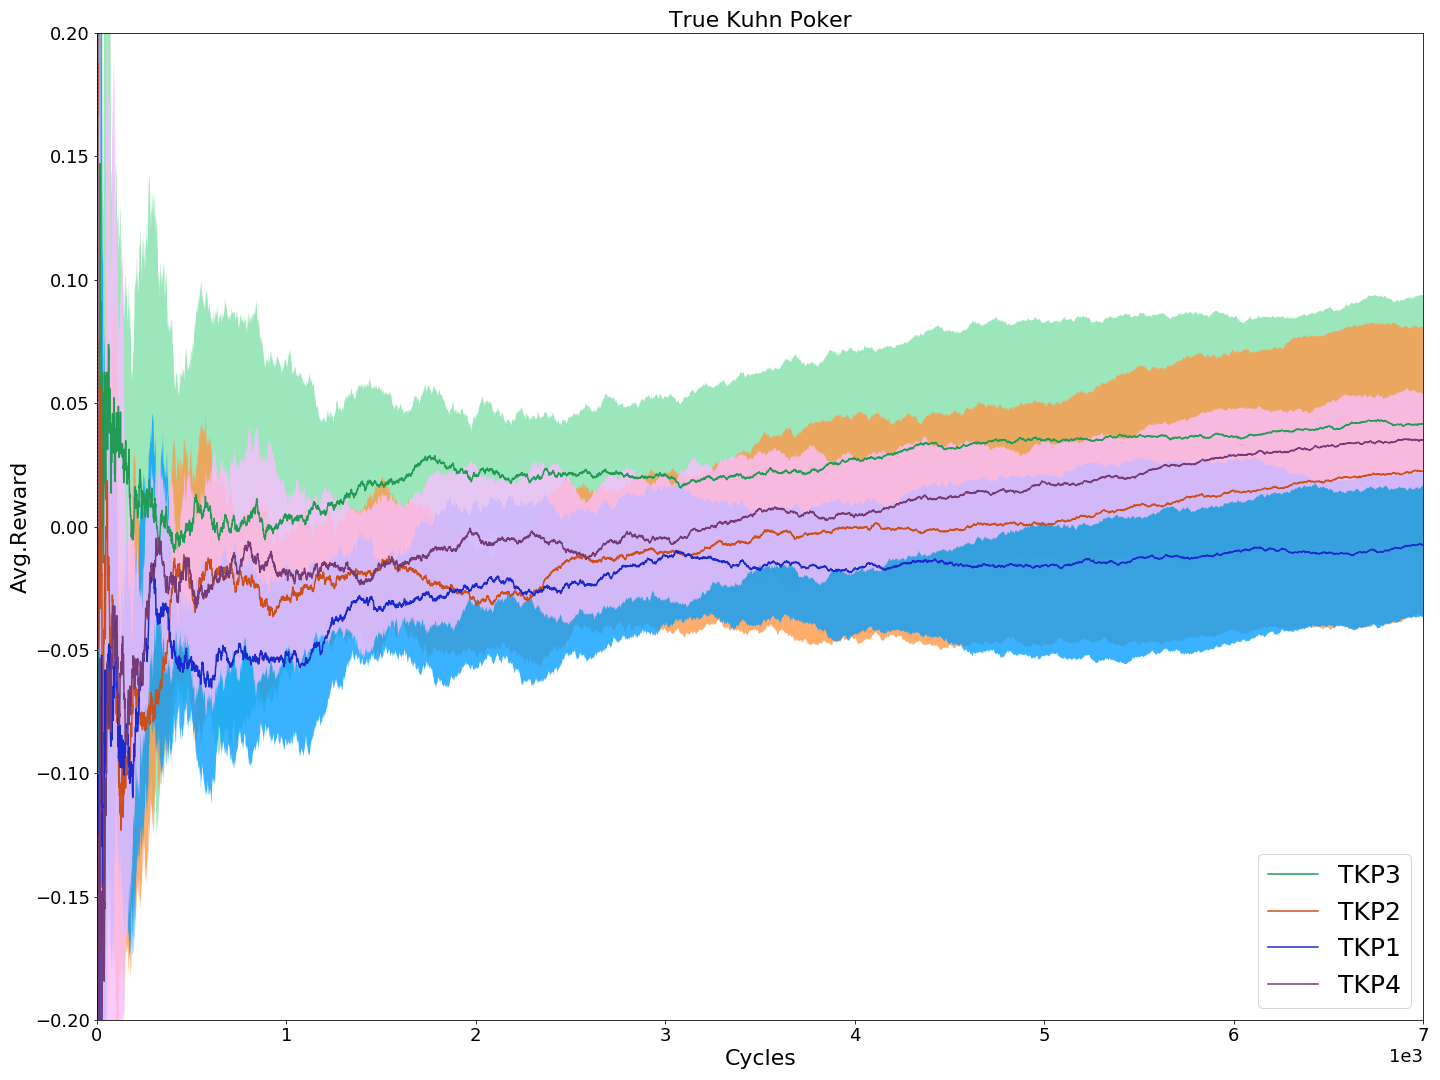
\includegraphics[width=9.1cm]{4_True_Kuhn_Poker}
\end{figure}

 \begin{figure}[h]
 \centering
    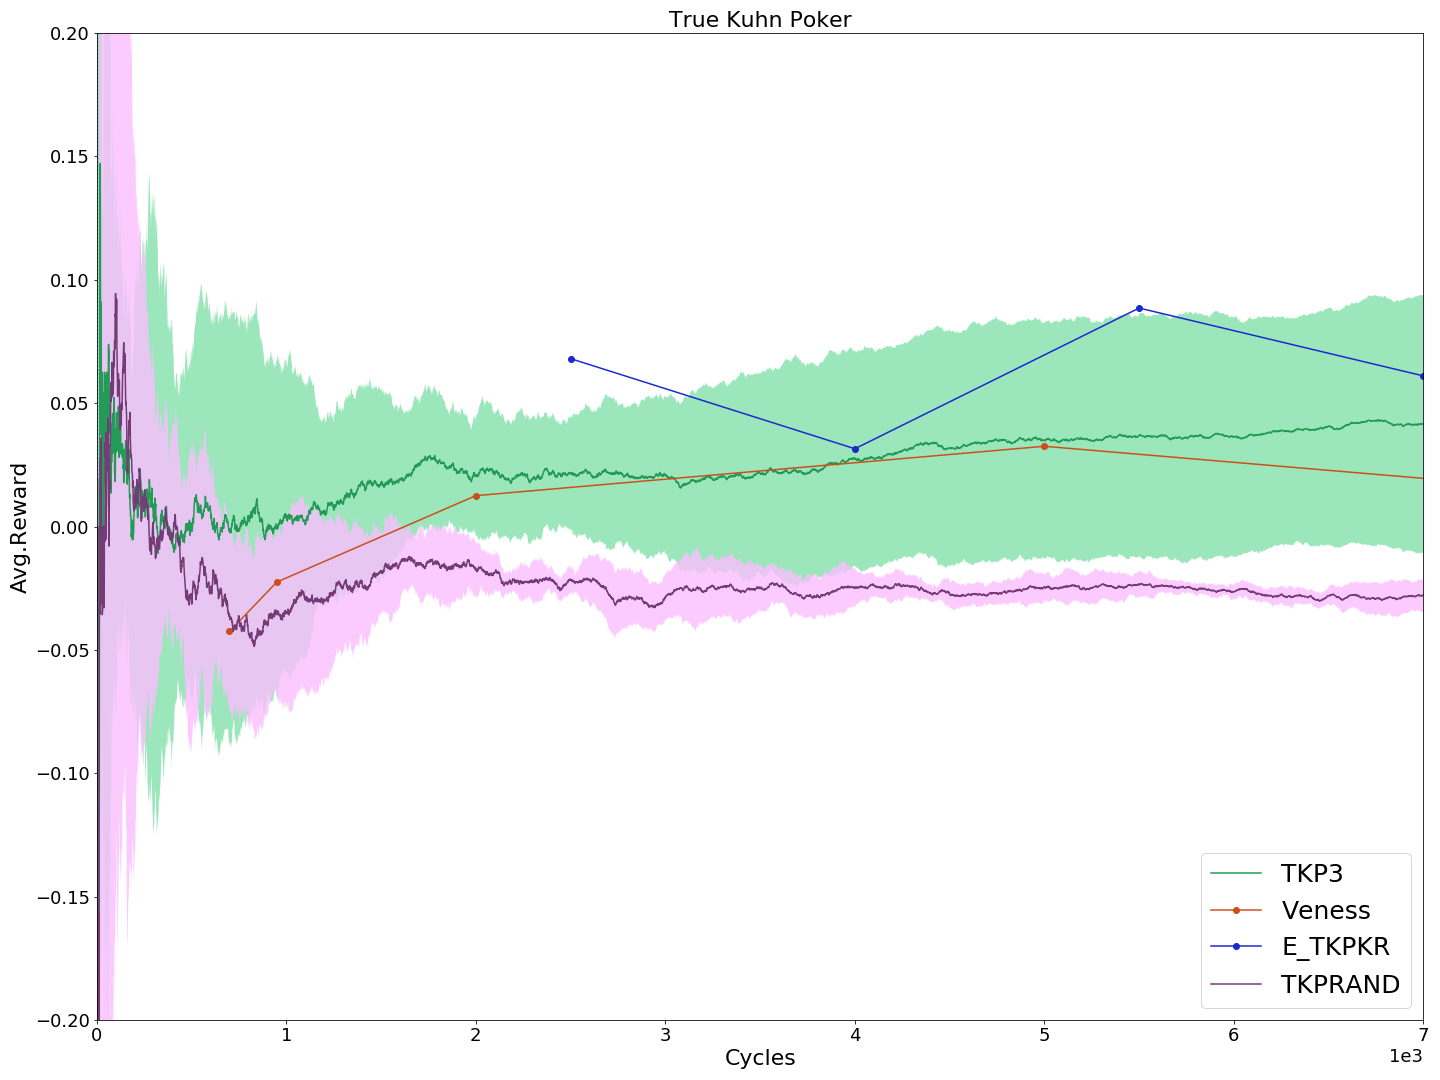
\includegraphics[width=9.1cm]{True_Kuhn_Poker}
\end{figure}

Compared to the random agent, our agent performed superiorly. Compared to \citep{veness2011monte} our agent performed similarly.

\newpage

\subsection{TicTacToe}
\begin{tabular}{|l|l|l|l|l|l|l|}
 \hline \centering
 Experiment ID& D & m & $\epsilon$ & $\gamma$ & Cycles & Average Reward \\ \hline
TTTE-1   & 64        & 9           & 0.9999      & 0.99991           & 145    & 0.0661625         \\ \hline
TTTE-2   & 96        & 9           & 0.9999      & 0.9995            & 24     & -0.636375         \\ \hline
% TicTacToe   & 256       & 9           & 0.9999      & 0.9991            & 13     &                \\
TTTE-4   & 128       & 10          & 0.9999      & 0.9991            & 12     & -0.83726875  \\  \hline  
E\underline{ }TTTE  & 64       & 9          & 0.9999      & 0.99991            & 180     & N/A  \\  \hline    
\end{tabular} 

 \begin{figure}[h]
 \centering
    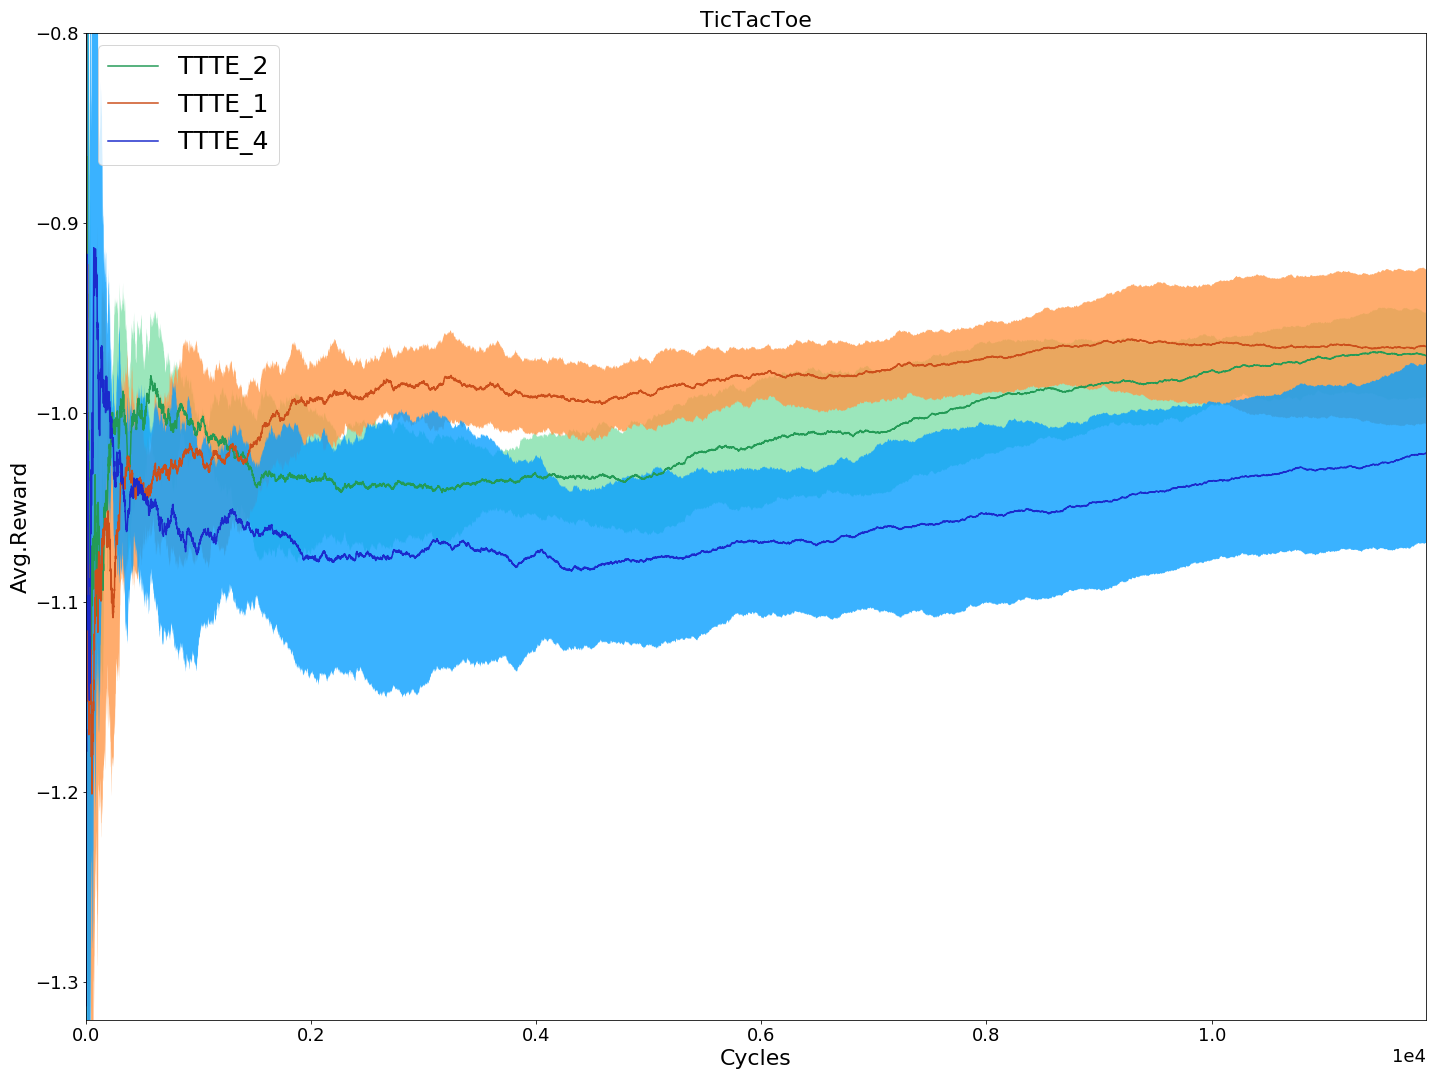
\includegraphics[width=9.1cm]{4_TicTacToe}
\end{figure}

 \begin{figure}[h]
 \centering
    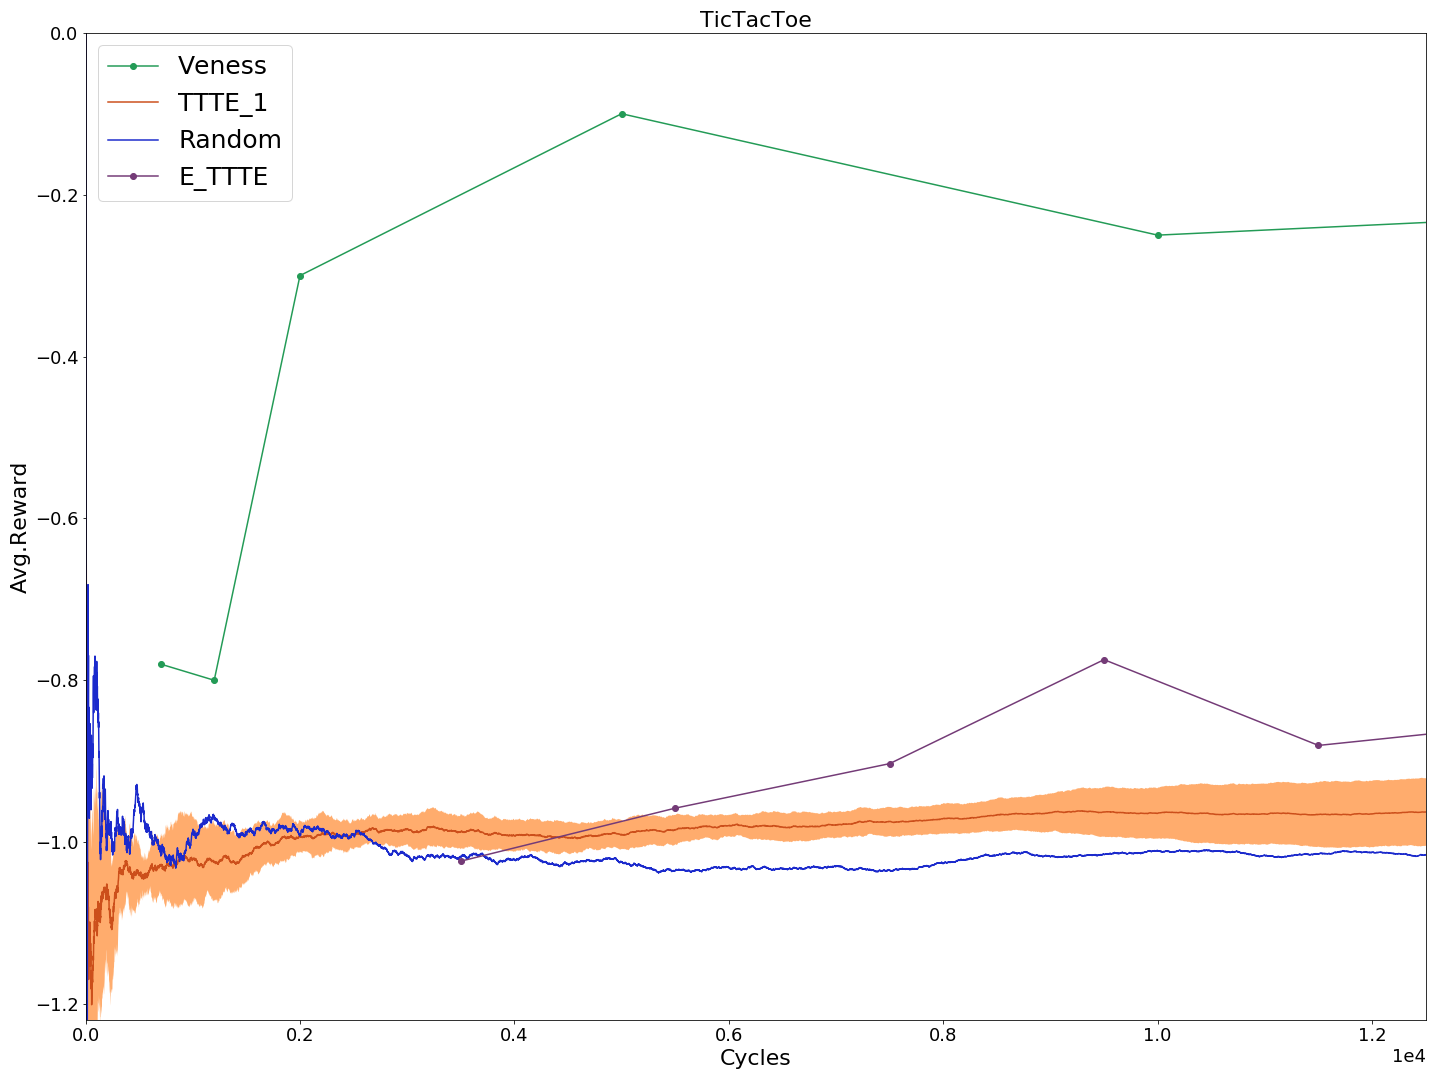
\includegraphics[width=9.1cm]{TicTacToe}
\end{figure}

Compared to the random agent, our agent performed slightly better. Compared to \citep{veness2011monte} our agent performed worse.

\newpage

\subsection{Extended Tiger}
 \begin{tabular}{|l|l|l|l|l|l|l|}
 \hline \centering
 Experiment ID& D & m & $\epsilon$ & $\gamma$ & Cycles & Average Reward \\ \hline
ETGR-1 & 96        & 4           & 0.999       & 0.99991           & 130    & -7.77525        \\ \hline
ETGR-2 & 64        & 4           & 0.999       & 0.999             & 12     & -7.08699       \\ \hline
ETGR-3 & 42        & 8           & 0.999       & 0.9991            & 13     & -10             \\ \hline
ETGR-4 & 256       & 4           & 0.999       & 0.9991            & 13     & -7.519  \\ \hline 
E\underline{ }ETGR & 64       & 4           & 0.999       & 0.999            & 15     & N/A  \\ \hline    
\end{tabular} 

 \begin{figure}[h]
 \centering
    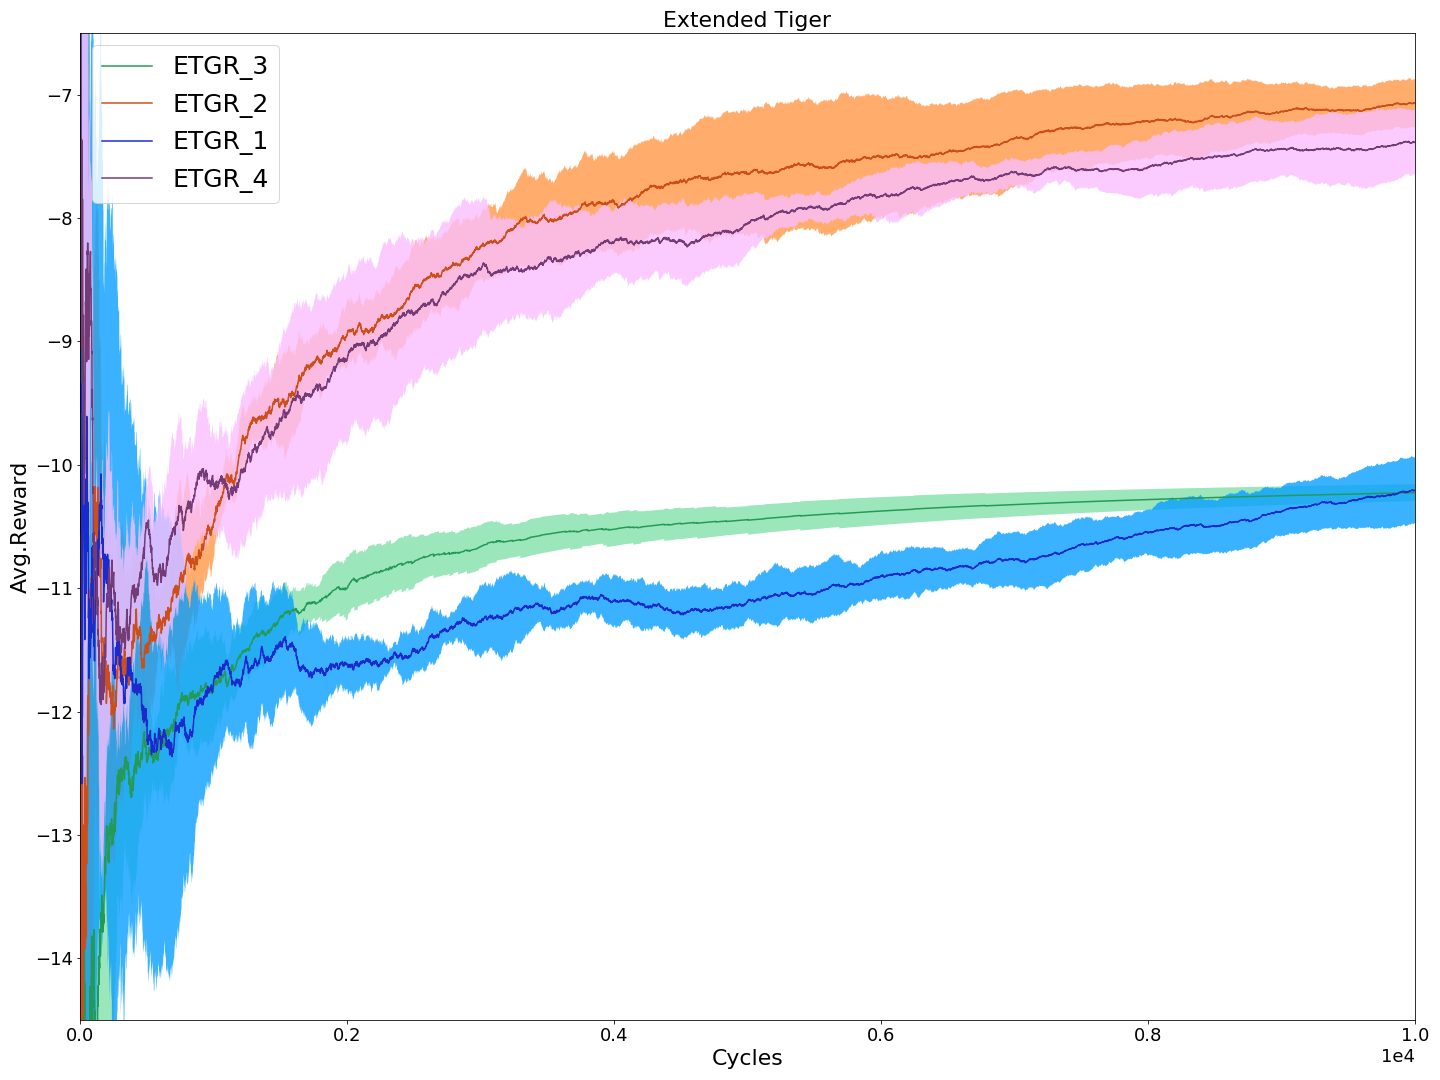
\includegraphics[width=9.1cm]{4_Extended_Tiger}
\end{figure}

 \begin{figure}[h]
 \centering
    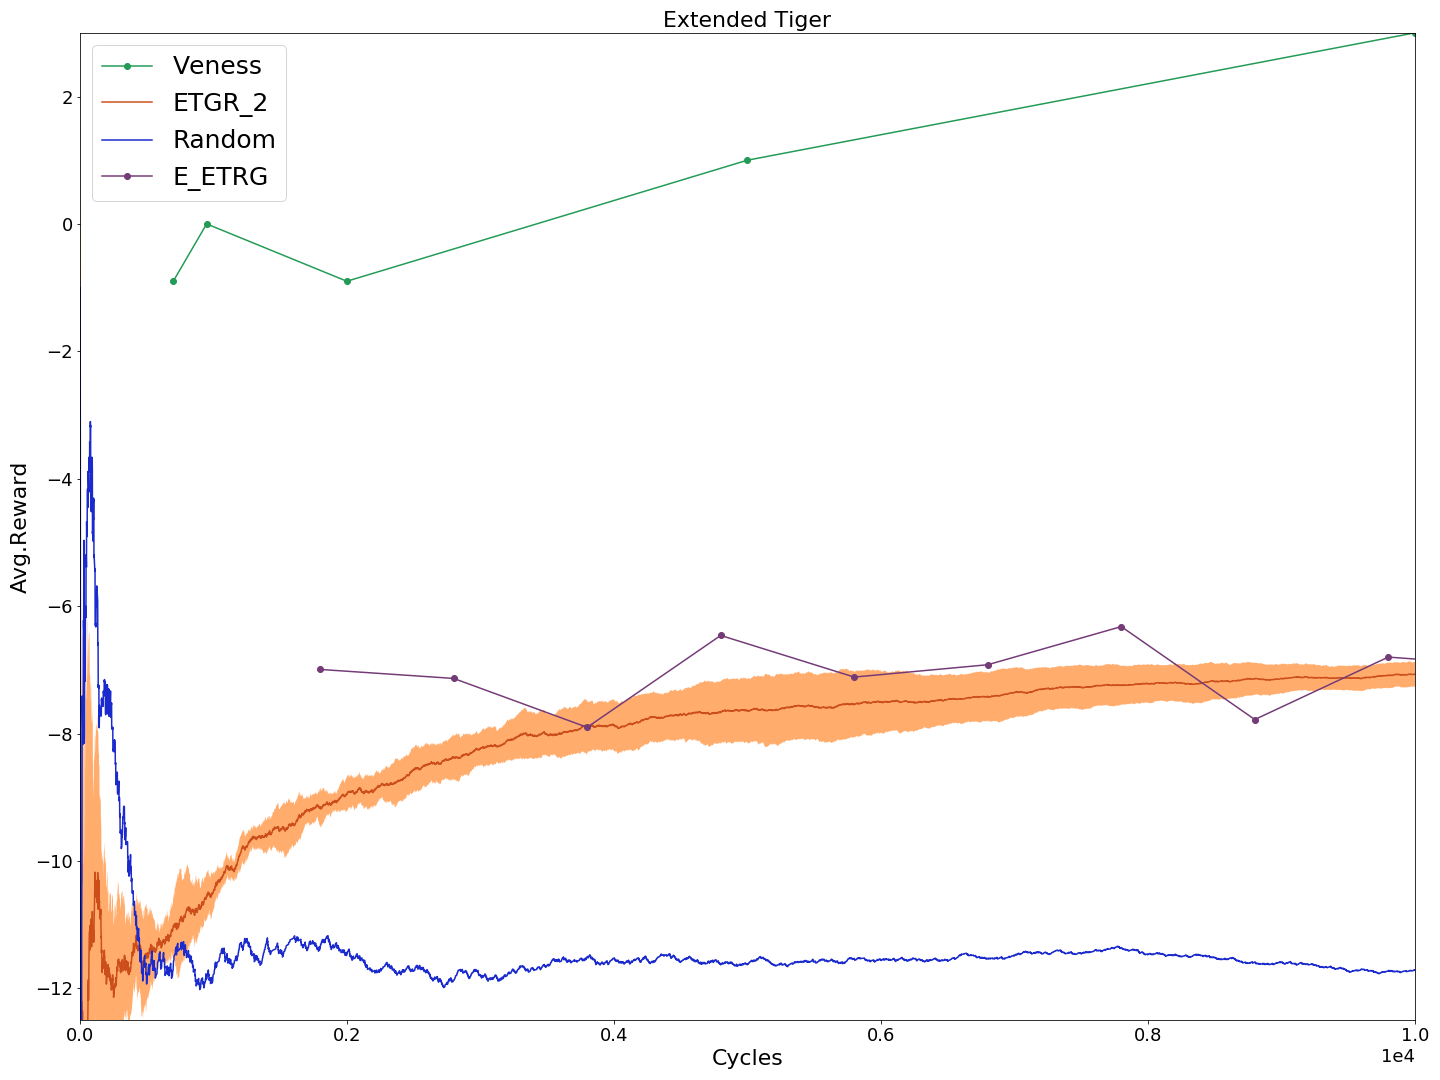
\includegraphics[width=9.1cm]{Extended_Tiger}
\end{figure}

Compared to the random agent, our agent performed superiorly. Compared to \citep{veness2011monte} our agent performed worse.

\newpage

\subsection{Pacman}
 \begin{tabular}{|l|l|l|l|l|l|l|}
 \hline \centering
 Experiment ID& D & m & $\epsilon$ & $\gamma$ & Cycles & Average Reward \\ \hline
PCMN-1  & 256       & 8           & 0.999       & 0.999             & 12     & -0.994        \\ \hline
%Pacman      & 512       & 10          & 0.9999      & 0.999             & 7      &                \\
 PCMN-3    & 256       & 4           & 0.999       & 0.9991            & 13     & -1.0055625       \\ \hline
 PCMN-4     & 92        & 4           & 0.999       & 0.999             & 7      &    -1.000225    \\  \hline 
  E\underline{ }PCMN    & 256        & 8           & 0.999       & 0.999             & 15      &    N/A    \\  \hline     
\end{tabular} \\

 \begin{figure}[h]
 \centering
    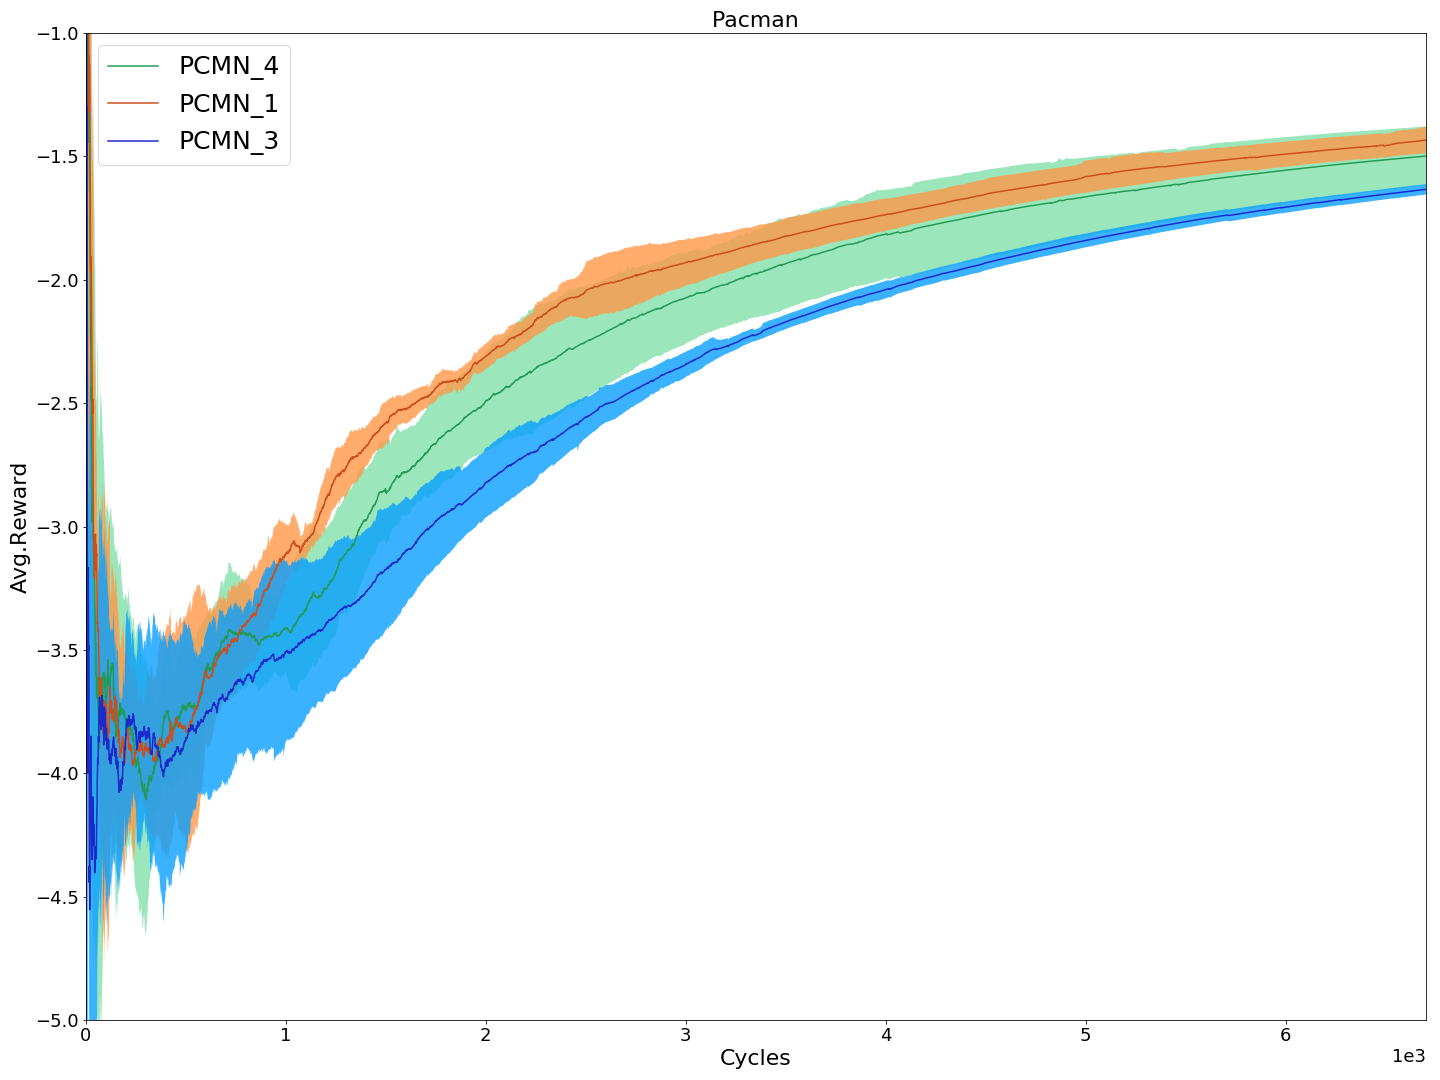
\includegraphics[width=9.1cm]{4_Pacman}
\end{figure}

 \begin{figure}[h]
 \centering
    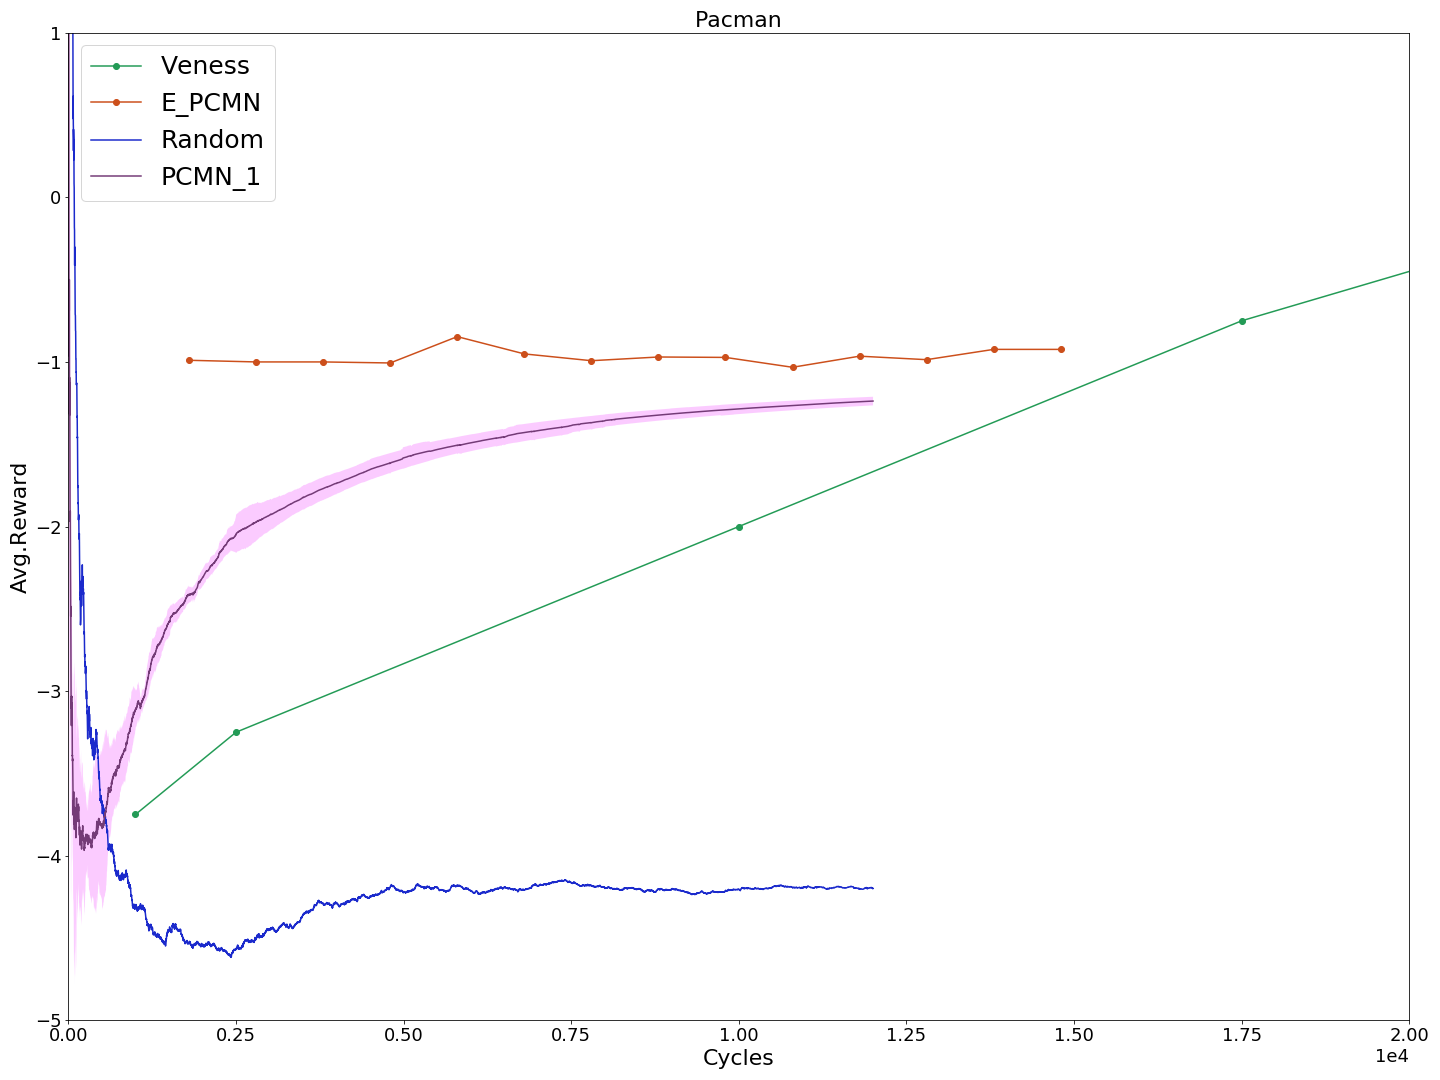
\includegraphics[width=9.1cm]{Pacman}
\end{figure}

Compared to the random agent, our agent performed superiorly. Compared to \citep{veness2011monte} our agent performed similarly.

\newpage


\subsection{Cross Domain-Kuhn Poker and BRPS }
 \begin{tabular}{|l|l|l|l|l|l|l|}
 \hline \centering
 Experiment ID& D & m & $\epsilon$ & $\gamma$ & Cycles (KP) & Cycles (BRPS) \\ \hline
BRPS\underline{ }KPKR  & 96       & 8           & 0.9999       & 0.9991             & 12    &  10      \\ \hline    
\end{tabular} \\

First\underline{ }BRPS is the initial training. Second\underline{ }KPKR is the cross domain running on Kuhn poker. Third\underline{ }BRPS is the evaluation for again running on Biased Rock Paper Scissors.


 \begin{figure}[h]
 \centering
    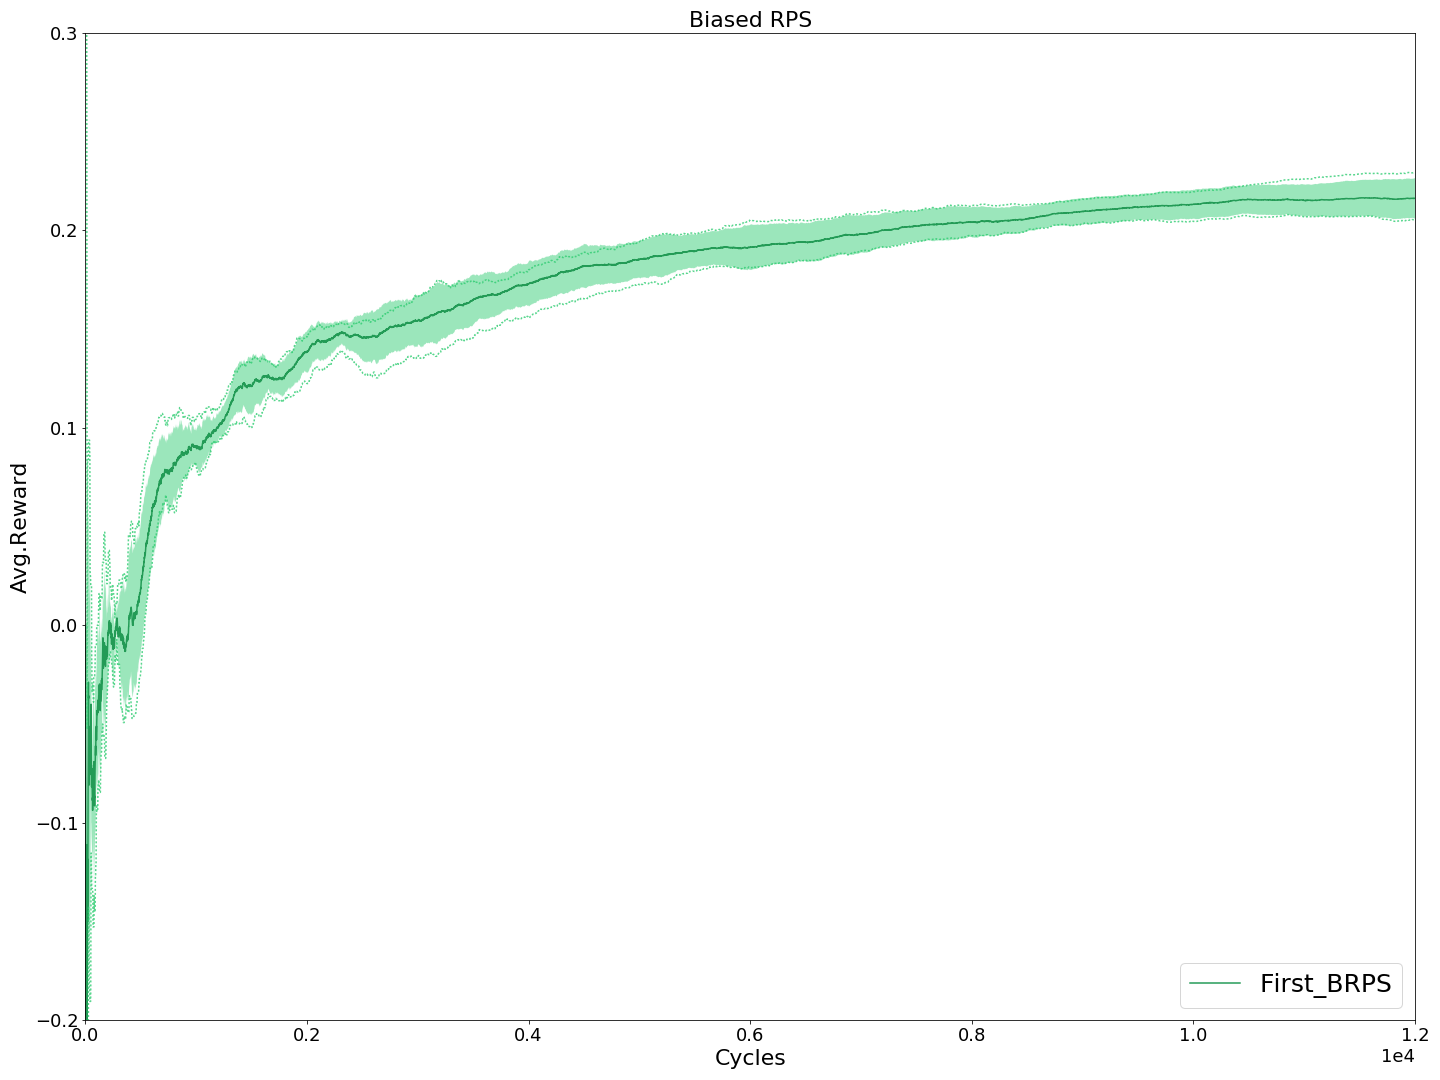
\includegraphics[width=9.1cm]{First_BRPS}
\end{figure}

\begin{figure}[h]
 \centering
    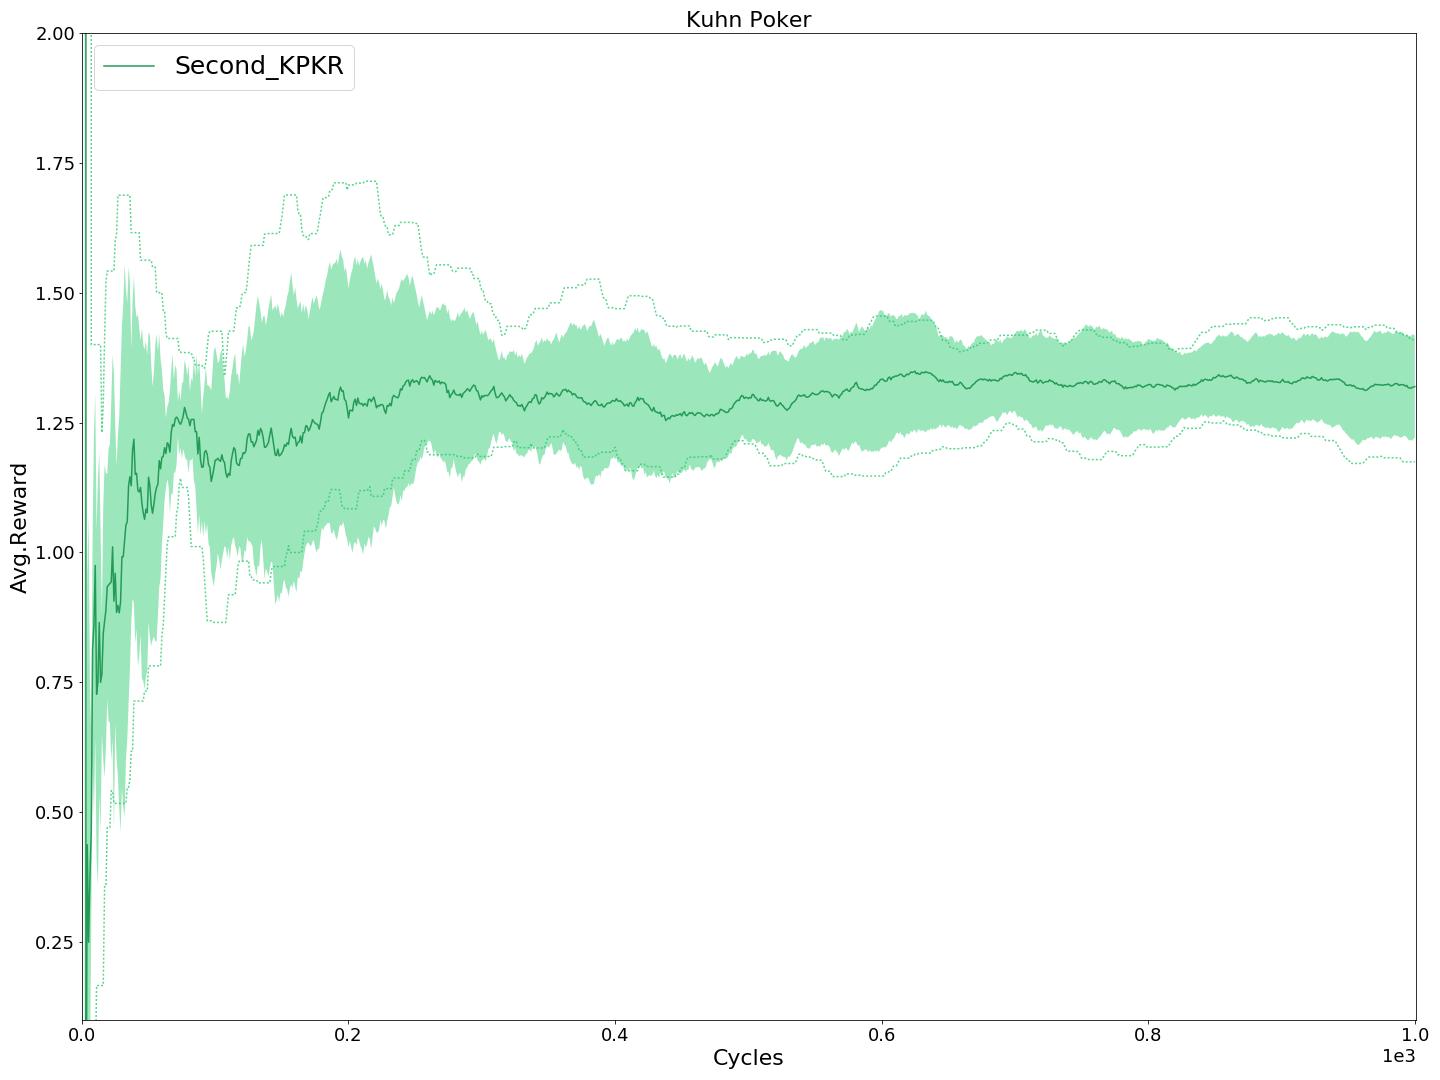
\includegraphics[width=9.1cm]{Second_KPKR}
\end{figure}

\begin{figure}[h]
 \centering
    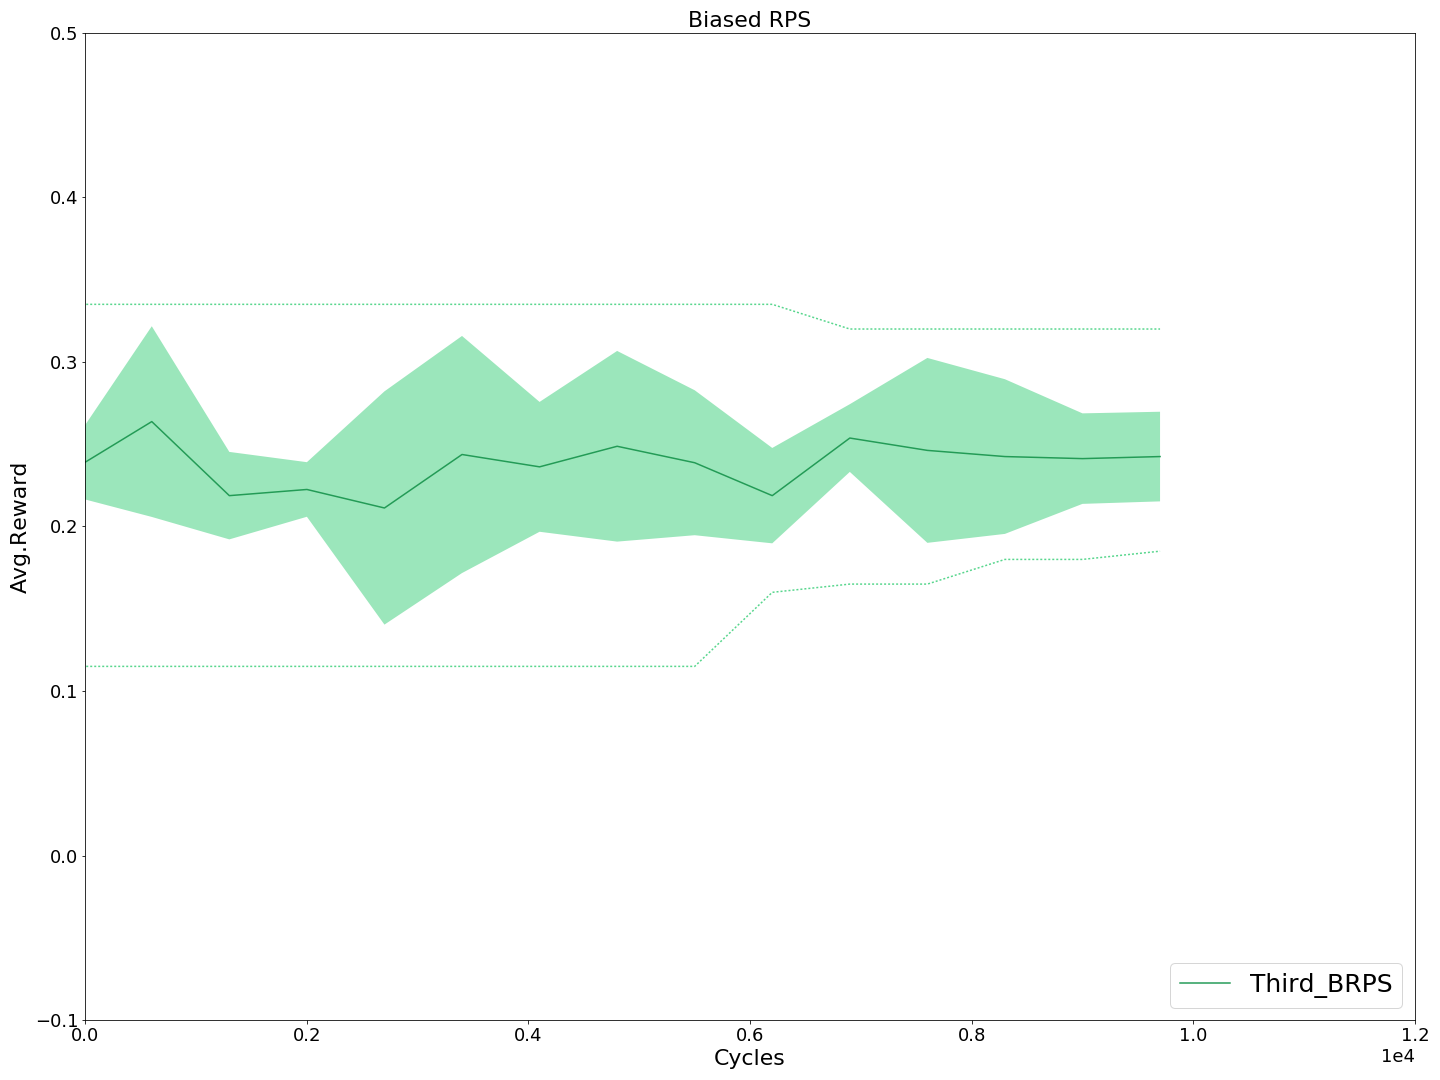
\includegraphics[width=9.1cm]{Third_BRPS}
\end{figure}


\newpage

\section{Discussion}


The main goal of our implementation of MC-AIXI-CTW was to achieved comparable results to \citep{veness2011monte} in the domains we chose. Due to computational constraints we did not use the exact same parameters for our agents in each environment. Regardless we were able to achieve our goal, and in each domain our agent had comparable performance. Although our plots did not exactly match those of \citep{veness2011monte}, especially for harder environments, after training our evaluation was comparable. \\

Modularity was another one of the goals with our implementation of MC-AIXI-CTW. With this in mind we managed to create a loosely coupled system in which each part can be replaced easily. For example, if we wished to use Context Tree Switching \citep{veness2012context} in the place of Context Tree Weighting then the implementation required is minimal. \\

Mentioned in \citep{veness2011monte}, the set up need not be in base 2. In fact, if base 3 was used then the observation space $|\mathcal{O}|$ of tictactoe would be reduced from $2^{18}=262144$ to $3^9 = 19683$. Reducing the observation space so much would lead to a much smaller history, and ultimately a speedup for the computation. Another possible speedup could come from reward scaling.  e.g. for extended tiger, scaling rewards of 0,90,99,130 to 0,9,10,13. This would reduce the reward bits from 8 to 4, and be an improvement to computation time. \\

Additionally we implements the True Kuhn Poker domain. That is the Kuhn Poker exactly as described in \citep{kuhn1950simplified}. This is different to the Kuhn Poker mentioned in  \citep{veness2011monte} in which the game is not zero sum. \\

Lastly we were able to implement was our agent in the RoboCup simulation environment. However, in this environment our agent was unable to outperform a random agent. This was likely due to the large search space of the environment. One way in which we may we able to reduce the size of the state space of RoboCup simulation (and possibly other environments) is through state aggregation. State aggregation is merging or aggregating equivalent or similar states to same states. State aggregation reduces the observation (and reward) space, thereby reducing search space, thereby reducing computation time.


\section{Conclusion}
We implemented and tested a version of the MC-AIXI-CTW agent presented by (Veness et al. 2011). The results of Veness and colleagues were not reproduced exactly, but our results are nonetheless similar enough to substantiate their claim that MC-AIXI-CTW can learn their domains.

In all the environments we tested our MC-AIXI-CTW agent was able to outperform a random agent. Near optimal to optimal solutions were achieved on on small domains. However, it runs into difficulty for larger domains, where care must be taken to manage the memory and initialize data structures as you go. This comes into play especially for TicTacToe, Pacman and Extended tiger. 

MC-AIXI-CTW is more than anything a proof of concept. The agent design may readily be improved by various methods. Multithreading is an obvious candidate. Future work may look into using Context Tree Switching in place of CTW, which we expect to lead to similar results with less computation time. The implementation of MCTS has been relatively bare-bones in that it failed to leverage the rich literature of improvements that has been developed since the technique's inception. Using our modular implementation of MC-AIXI-CTW as a basis, the next step would be to develop the ideas of Veness and colleagues to their full potential as a solution to the general reinforcement learning problem. 

\printbibliography



\end{document}
